
%
%%%%%%%%%%%%%%%%%%%%%%%%%
%                       %
% Problem Formulation   %
%                       %
%%%%%%%%%%%%%%%%%%%%%%%%%
%
% Brief abstract: formulates the two problem (coverage, (re)planning)
%
% Completion (1-10): 10
% Missing: none, but further consistency check is needed
%
\chapter{Problem Formulation}
\label{cp:pb}

\begin{chapquote}{\cite{arkin2001optimal}}
  ``While we will often speak of the [coverage] problem as `milling' with a `cutter', many of its important applications arise in various contexts outside of machining.''
\end{chapquote}

\vspace*{1em}

\lettrine{I}{n this chapter}, we discuss the planning and coverage problems that we are interested in solving. The coverage problem is the problem of finding the path that covers all the points in a given space, for instance, the agricultural field in \fref{sec:motivation}{Section}. The coverage path with some user-defined computations forms the plan. The planning problem is then the problem of replanning the plan. It is replanned energy-wise in the eventuality of energy constraints dissatisfaction, and whenever the uncertainty affects the flight unexpectedly. To define both the problems, we need some basic constructs. In particular, we provide formal definitions in \fref{sec:definitions}{Sections}\fref{sec:defs-stages-triggs}{--\hspace*{-.8ex}} that include the computations, motion, computations energy, and motion energy. We then define the difference between computations and motion energy (\Gls{acr:mace}), which we encountered in \fref{sec:aerial-robo-types}{Section}, path, and other plan-specific constructs. We then use all these to formulate the planning and coverage problems in \fref{sec:plan-pb}{Section}. We illustrate the problem with an example of the precision agriculture scenario in \fref{sec:flight-plan}{Section}.

In \fref{cp:dyn}{Chapter}, we propose two algorithms. A first algorithm generates the coverage path, and another algorithm replans the plan in time, solving the coverage and planning problems. The replanning is energy-aware: the algorithm outputs the best trajectory of the path and computations alteration for an aerial robot with varying battery and atmospheric conditions. 

The chapter connects to the remainder of this work as follows. Here we formalize the plan, the planning and coverage problems, and some other basic constructs. We use the plan characteristics to derive an energy model in \fref{cp:model}{Chapter}, which we estimate from measured data in \fref{cp:opt}{Chapter}. We solve the planning problem using modern optimal control techniques and the coverage problem using a planning algorithm in \fref{cp:dyn}{Chapter}. With the solution to the coverage and planning problem, we output an initial plan, and refine the plan in terms of the path and computations. We guide the aerial robot using a vector field, where we use the plan's building blocks from this chapter. We discuss past approaches to solve the planning problem in \fref{cp:soa}{Chapter} and the concrete implementation in \fref{app:imp}{Appendix}.


%%%%%%%%%%%%%%%%%%%%%%%%%%%%%%%%%%%%%%%%%%%%%%%%
\section{Definitions of computations and motion}
\label{sec:definitions}

Firstly, we define computations, motion, their energy, and M\&CE. Our dynamic planning depends on these basic concepts.

\begin{highlight}
  \begin{defn}[Computations/motion]\label{def:comps}
    \emph{Computations}\findex{computations} are energy-demanding computational tasks. The aerial robot runs the computations on heterogeneous computing hardware that interfaces microcontrollers.
    
    \emph{Motion}\findex{motion} is the act of the aerial robot moving in the surrounding environment. The aerial robot runs some primitives on microcontrollers that interface actuators, motors, and other components.
  \end{defn}
\end{highlight}

Autonomous capabilities are often achieved by interconnecting heterogeneous computing hardware and microcontrollers. We assume for the computations that the heterogeneous computing hardware runs a schedule characterized by some parameters. For instance, for the CNN detection from the precision agriculture scenario in \fref{sec:objective}{Section}, a parameter is the frames per second (\Gls{acr:fps})\findex{frames per second} rate. Alike for the computations, we assume for the motion that the robot travels some paths characterized by some other parameters. For instance, for the coverage, a parameter changes the distance between the survey lines.

\begin{highlight}
\begin{defn}[Computations/motion and overall energy]\label{def:comp-mot-energy}
  Given a path characterized by $\rho$ parameters $c_i^\rho:=\{c_{i,1},c_{i,2},\dots,c_{i,\rho}\}$, the \emph{motion energy}\findex{motion energy} is the energy spent by the aerial robot while moving on the path.

  Given a schedule characterized by parameters $c_i^\sigma:=\{c_{i,\rho+1},c_{i,\rho+2},\dots,c_{i,\rho+\sigma}\}$, the \emph{computations energy}\findex{computations energy} is the energy spent by heterogeneous computing hardware executing the schedule.

  The \emph{overall energy}\findex{overall energy} is the sum of motion energy and computations energy.
\end{defn}
\end{highlight}

Physically, motion energy is the energy spent by all the systems powering the aerial robot, excluding the heterogeneous computing hardware. We use watts for instantaneous or average measures of computations, motion, and overall energies, whereas joules for measures over a given time interval. We show in \fref{sec:defs-stages-triggs}{Section} what we mean by the characterization of paths and computations with some parameters.

\Gls{acr:mace}\findex{difference of motion and computations energy} that we introduced in \fref{sec:aerial-robo-types}{Section} is the difference between average motion and computations energy. It is measured in watts, and it gives a measure of which of the two energy components is predominant. For \Gls{acr:mace} greater than zero, the motion energy dominates over the computations. The dynamic planning approach plans first an energy-efficient path. If we return briefly to \fref{fig:robots-vs-power}{Figure}, it is the case for rotary-wing aerial robots \sref{lab:matrice} and \sref{lab:agras}. On the contrary, for \Gls{acr:mace} lower than zero, the computations energy dominates. The dynamic planning approach plans first a power-saving schedule. It is the case for the lighter-than-air aerial robot \sref{lab:skye} in \fref{fig:robots-vs-power}{Figure}. For \Gls{acr:mace} close to zero, both energy components are important energy-wise. The dynamic planning approach plans both an energy-efficient path and a power-saving schedule to a similar extent. This M\&CE is characteristic of fixed-wing aerial robots, such as \sref{lab:cumulus}\fref{lab:opterra}{--\hspace*{-.8ex}} in \fref{fig:robots-vs-power}{Figure}.


%%%%%%%%%%%%%%%%%%%%%%%%%%%%%%%%%%%%%%%
\section{Definition of path functions}
\label{sec:path-functions}

To model the path, we use multiple mathematical functions $\varphi_1,\varphi_2,\dots$ that we call path functions. These functions express the path in 2D space at an altitude $h\in\mathbb{R}$ for an inertial navigation frame $\mathcal{O}_W$. We discuss a generalization of the path functions in 3D space and how it affects the guidance in \fref{cp:conc}{Chapter}. 

\begin{highlight}
  \begin{defn}[Path functions]\label{def:paths}
    $\varphi_i:\mathbb{R}^2\rightarrow\mathbb{R},\,\forall i\in\{1,2,\dots\}$ are \emph{path functions}\findex{path functions} used to model the path. They are a function of a generic time-dependent point $\mathbf{p}(t):=(x_{\mathbf{p}(t)},y_{\mathbf{p}(t)})$ of the aerial robot flying in the 2D space and are continuous and twice differentiable. 
  \end{defn}
\end{highlight}

\begin{figure}[t!]
  \centering
  
\definecolor{cECECEC}{RGB}{236,236,236}
\definecolor{c989898}{RGB}{152,152,152}
\small

\def \globalscale {1.000000}
\begin{tikzpicture}[y=0.80pt, x=0.80pt, yscale=-.9*\globalscale, xscale=.9*\globalscale, inner sep=0pt, outer sep=0pt]
\path[fill=cECECEC,line join=round,line width=0.160pt] (338.3020,263.8010) -- (381.1050,-0.0001) -- (102.8640,12.1601) -- (58.1440,275.9610) -- (338.3020,263.8010) -- cycle;



\path[draw=c989898,line join=round,line width=0.512pt] (147.6250,213.3720) -- (173.5250,186.3120) -- (132.2780,180.7850);



\path[fill=c989898,line join=round,line width=0.256pt] (163.3290,190.5470) -- (158.3650,192.4980) -- (158.1310,191.9020) -- (163.0950,189.9520) -- (163.3290,190.5470) -- cycle(153.4020,194.4490) -- (148.4380,196.4000) -- (148.2040,195.8040) -- (153.1680,193.8530) -- (153.4020,194.4490) -- cycle(143.4740,198.3510) -- (138.5110,200.3020) -- (138.2760,199.7060) -- (143.2400,197.7550) -- (143.4740,198.3510) -- cycle(133.5470,202.2530) -- (128.5830,204.2040) -- (128.3490,203.6080) -- (133.3130,201.6570) -- (133.5470,202.2530) -- cycle(123.6200,206.1550) -- (118.6560,208.1060) -- (118.4220,207.5100) -- (123.3850,205.5590) -- (123.6200,206.1550) -- cycle(113.6920,210.0560) -- (108.7280,212.0070) -- (108.4940,211.4120) -- (113.4580,209.4610) -- (113.6920,210.0560) -- cycle(103.7650,213.9580) -- (100.0090,215.4350) -- (99.7748,214.8390) -- (103.5310,213.3630) -- (103.7650,213.9580) -- cycle(173.2570,186.6450) -- (168.2930,188.5960) -- (168.0590,188.0010) -- (173.0220,186.0500) -- (173.2570,186.6450) -- cycle;



\path[draw=c989898,line join=round,line width=0.512pt] (55.1846,208.3180) -- (99.4269,215.2590);



\path[draw=black,line join=round,line width=0.512pt] (68.2145,216.7950) -- (99.1080,215.5400);



\path[draw=c989898,line join=round,line width=0.512pt] (99.5793,215.0880) -- (196.7320,112.9950);



\path[draw=foo,line join=round,line width=0.512pt] (139.9040,221.4650) -- (147.6230,213.4870);



\path[draw=black,line join=round,line width=0.512pt] (99.6097,215.3190) -- (377.1250,258.8550);



\path[fill=foo,line join=round,line width=0.256pt] (163.7520,67.1159) -- (158.7880,69.0661) -- (158.5540,68.4704) -- (163.5180,66.5202) -- (163.7520,67.1159) -- cycle(153.8240,71.0164) -- (148.8600,72.9667) -- (148.6260,72.3709) -- (153.5900,70.4207) -- (153.8240,71.0164) -- cycle(143.8960,74.9168) -- (138.9320,76.8670) -- (138.6980,76.2713) -- (143.6620,74.3211) -- (143.8960,74.9168) -- cycle(133.9680,78.8173) -- (129.0040,80.7676) -- (128.7700,80.1719) -- (133.7340,78.2216) -- (133.9680,78.8173) -- cycle(124.0400,82.7178) -- (119.0760,84.6679) -- (118.8420,84.0722) -- (123.8060,82.1220) -- (124.0400,82.7178) -- cycle(114.1120,86.6182) -- (109.1480,88.5685) -- (108.9140,87.9728) -- (113.8780,86.0225) -- (114.1120,86.6182) -- cycle(104.1840,90.5187) -- (99.9651,92.1761) -- (99.7311,91.5804) -- (103.9500,89.9230) -- (104.1840,90.5187) -- cycle(173.6800,63.2155) -- (168.7160,65.1657) -- (168.4820,64.5700) -- (173.4460,62.6198) -- (173.6800,63.2155) -- cycle;



\path[draw=black,line join=round,line width=0.512pt] (99.6290,215.7460) -- (99.6701,45.2765);



\path[fill=black,line join=round,line width=0.160pt] (97.4234,50.0749) -- (99.6963,48.0699) -- (101.7800,50.0657) -- (99.5939,44.2973) -- (97.4234,50.0749) -- cycle;



\path[fill=black,line join=round,line width=0.160pt] (372.7840,255.6340) -- (374.2970,258.2610) -- (371.9260,259.9050) -- (378.0140,258.9110) -- (372.7840,255.6340) -- cycle;



\path[draw=c989898,fill=c989898,line join=round,line width=0.160pt] (191.9960,115.1180) -- (195.0250,115.0410) -- (195.3410,117.9090) -- (197.3700,112.0830) -- (191.9960,115.1180) -- cycle;



\path[draw=black,line join=round,line width=0.512pt] (99.6614,215.4240) -- (348.2110,205.3130);



\path[fill=black,line join=round,line width=0.256pt] (365.8960,204.3560) -- (371.2240,204.1220) -- (371.2520,204.7610) -- (365.9240,204.9950) -- (365.8960,204.3560) -- cycle(376.5520,203.8870) -- (381.8800,203.6530) -- (381.9080,204.2920) -- (376.5800,204.5270) -- (376.5520,203.8870) -- cycle(387.2080,203.4190) -- (391.6130,203.2250) -- (391.6410,203.8640) -- (387.2370,204.0580) -- (387.2080,203.4190) -- cycle(355.2390,204.8250) -- (360.5670,204.5900) -- (360.5960,205.2300) -- (355.2670,205.4640) -- (355.2390,204.8250) -- cycle;



\path[fill=black,line join=round,line width=0.256pt] (51.6916,217.8380) -- (46.3616,218.0290) -- (46.3388,217.3890) -- (51.6687,217.1990) -- (51.6916,217.8380) -- cycle(41.0317,218.2190) -- (35.7017,218.4090) -- (35.6789,217.7700) -- (41.0088,217.5790) -- (41.0317,218.2190) -- cycle(30.3718,218.6000) -- (25.0419,218.7900) -- (25.0190,218.1500) -- (30.3490,217.9600) -- (30.3718,218.6000) -- cycle(62.3514,217.4570) -- (57.0215,217.6480) -- (56.9986,217.0080) -- (62.3286,216.8180) -- (62.3514,217.4570) -- cycle;



\path[draw=black,line join=round,line width=0.512pt] (138.1150,223.3150) -- (140.0590,221.3710);



\path[draw=c989898,line join=round,line width=0.512pt] (129.6630,180.5070) -- (132.3930,180.8300);



\path[draw=c989898,line join=round,line width=0.512pt] (173.5260,186.3500) -- (173.5730,63.0377);



\path[draw=black,line join=round,line width=0.512pt] (96.7492,91.8181) -- (99.4988,91.8249);



\path[cm={{1.0,0.0,0.0,1.0,(376.0,276.0)}}] (0.0000,0.0000) node[above right] () {$x$};



\path[cm={{1.0,0.0,0.0,1.0,(198.0,102.0)}}] (0.0000,0.0000) node[above right] () {$y$};



\path[cm={{1.0,0.0,0.0,1.0,(85.0,46.0)}}] (0.0000,0.0000) node[above right] () {$z$};



\path[draw=black,line join=round,line width=0.512pt] (83.3760,232.1090) -- (99.6032,215.0620);



\path[fill=c989898,line join=round,line width=0.512pt] (173.2360,184.7230) .. controls (174.0900,184.7230) and (174.7820,185.4150) .. (174.7820,186.2700) .. controls (174.7820,187.1240) and (174.0900,187.8160) .. (173.2360,187.8160) .. controls (172.3810,187.8160) and (171.6890,187.1240) .. (171.6890,186.2700) .. controls (171.6890,185.4150) and (172.3810,184.7230) .. (173.2360,184.7230) -- cycle;



\path[cm={{1.0,0.0,0.0,1.0,(161.0,289.0)}}] (0.0000,0.0000) node[above right] () {$\varphi(x,y):=2y-x$};



\path[cm={{1.0,0.0,0.0,1.0,(353.0,224.0)}}] (0.0000,0.0000) node[above right] () {$2y-x=h$};



\path[cm={{1.0,0.0,0.0,1.0,(131.0,238.0)}}] (0.0000,0.0000) node[above right] () {$x_\mathbf{p}$};



\path[cm={{1.0,0.0,0.0,1.0,(113.0,180.9)}}] (0.0000,0.0000) node[above right] () {$y_\mathbf{p}$};



\path[cm={{1.0,0.0,0.0,1.0,(41.0,98.0)}}] (0.0000,0.0000) node[above right] () {$\varphi(\mathbf{p})=d$};



\path[draw=c989898,fill=c989898,line join=round,line width=0.160pt] (175.7670,179.7880) -- (173.4940,181.7930) -- (171.4110,179.7970) -- (173.5970,185.5660) -- (175.7670,179.7880) -- cycle;



\path[draw=c989898,fill=c989898,line join=round,line width=0.160pt] (171.2840,70.1412) -- (173.5570,68.1363) -- (175.6400,70.1321) -- (173.4540,64.3637) -- (171.2840,70.1412) -- cycle;



\path[fill=foo,line join=round,line width=0.512pt] (173.4160,61.7418) .. controls (174.2700,61.7418) and (174.9630,62.4342) .. (174.9630,63.2885) .. controls (174.9630,64.1427) and (174.2700,64.8351) .. (173.4160,64.8351) .. controls (172.5620,64.8351) and (171.8700,64.1427) .. (171.8700,63.2885) .. controls (171.8700,62.4342) and (172.5620,61.7418) .. (173.4160,61.7418) -- cycle;



  \path[fill=cECECEC,line join=round,line width=0.160pt] (182.5940,102.1690) -- (164.2430,102.1690) -- (164.1940,119.9680) -- (182.5870,119.9220) -- (182.5940,102.1690) -- cycle;



  \path[cm={{1.0,0.0,0.0,1.0,(170.0,116.0)}}] (0.0000,0.0000) node[above right] () {$d$};



\path[cm={{1.0,0.0,0.0,1.0,(187.0,186.0)}}] (0.0000,0.0000) node[above right] () {$(x_\mathbf{p},y_\mathbf{p},h)$};


\path[draw=c989898,line join=round,line width=0.512pt] (99.6154,255.8180) -- (99.6251,215.7290);


\end{tikzpicture}


  \caption[Concept of a line as a path function]{The path is mathematical function $\varphi(\mathbf{p}(t))=h$ that represents a line at an altitude $h$. A generic point $\mathbf{p}$ in 2D space intersects the plane formed by $\varphi$ at a given value $d$ of the $z$-axis.}
  \label{fig:line-pf}
\end{figure}

\begin{figure}[t!]
  \centering
  
\definecolor{c989898}{RGB}{152,152,152}
\definecolor{cFFFFFF}{RGB}{255,255,255}
\small

\def \globalscale {1.000000}
\begin{tikzpicture}[y=0.80pt, x=0.80pt, yscale=-\globalscale, xscale=\globalscale, inner sep=0pt, outer sep=0pt]

\path[cm={{1.0,0.0,0.0,1.0,(0,0)}}] (10.0000,23.0000) node[below right] () {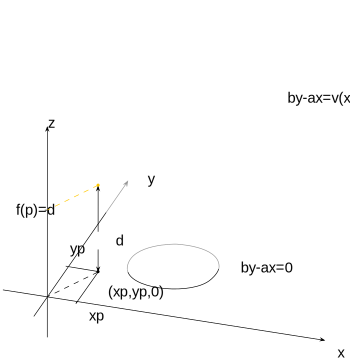
\includegraphics{figures/source/plot11}};


\path[draw=black,line join=round,line width=0.512pt] (2.8949,290.3560) -- (47.1372,297.2970);



\path[draw=black,line join=round,line width=0.512pt] (47.3200,297.3570) -- (324.8360,340.8930);



\path[draw=black,line join=round,line width=0.512pt] (47.3393,297.7850) -- (47.3804,127.3150);



\path[draw=black,line join=round,line width=0.512pt] (47.3257,337.8570) -- (47.3354,297.7680);



\path[draw=black,line join=round,line width=0.512pt] (47.2678,297.6320) -- (106.3620,212.7130);



\path[draw=c989898,line join=round,line width=0.512pt] (106.3620,212.7130) -- (127.7670,181.9530);



\path[fill=black,line join=round,line width=0.160pt] (45.1337,132.1130) -- (47.4066,130.1080) -- (49.4901,132.1040) -- (47.3042,126.3360) -- (45.1337,132.1130) -- cycle;



\path[fill=black,line join=round,line width=0.160pt] (320.4950,337.6720) -- (322.0070,340.2990) -- (319.6360,341.9440) -- (325.7240,340.9500) -- (320.4950,337.6720) -- cycle;



\path[cm={{1.0,0.0,0.0,1.0,(323.0,358.0)}}] (0.0000,0.0000) node[above right] () {$x$};



\path[cm={{1.0,0.0,0.0,1.0,(33.0,128.0)}}] (0.0000,0.0000) node[above right] () {$z$};



\path[cm={{1.0,0.0,0.0,1.0,(133.0,184.0)}}] (0.0000,0.0000) node[above right] () {$y$};



\path[draw=c989898,fill=c989898,line join=round,line width=0.160pt] (123.4090,184.7720) -- (126.3910,184.2350) -- (127.1390,187.0210) -- (128.2590,180.9550) -- (123.4090,184.7720) -- cycle;



\path[draw=black,line join=round,line width=0.512pt] (33.8410,316.9190) -- (47.2875,297.6020);



\path[draw=c989898,line join=round,line width=0.512pt] (219.3400,268.1300) .. controls (219.4020,267.7210) and (219.4350,267.3120) .. (219.4350,266.9020) .. controls (219.4350,246.0390) and (175.9680,244.5180) .. (175.9680,244.5180) .. controls (175.9680,244.5180) and (131.4840,243.8660) .. (127.5750,266.9020) .. controls (127.3910,267.9820) and (127.3660,269.0270) .. (127.4870,270.0360);



\path[draw=c989898,line join=round,line width=0.512pt] (127.4870,270.0360) .. controls (127.5930,270.9220) and (127.8120,271.7810) .. (128.1350,272.6120);



\path[draw=black,line join=round,line width=0.512pt] (128.1350,272.6120) .. controls (135.2830,291.0080) and (193.4860,295.5780) .. (210.9770,280.0880) .. controls (210.9770,280.0880) and (217.3970,275.0510) .. (219.0510,269.4220);



\path[draw=c989898,line join=round,line width=0.512pt] (219.0510,269.4220) .. controls (219.1760,268.9940) and (219.2750,268.5630) .. (219.3400,268.1300);



\path[draw=black,line join=round,line width=0.512pt] (76.1806,303.7580) -- (98.6304,272.0580) -- (68.5307,267.0880);



\path[fill=black,line join=round,line width=0.256pt] (88.4047,277.5740) -- (83.6131,279.9160) -- (83.3321,279.3410) -- (88.1237,276.9990) -- (88.4047,277.5740) -- cycle(78.8215,282.2580) -- (74.0299,284.6000) -- (73.7488,284.0250) -- (78.5405,281.6830) -- (78.8215,282.2580) -- cycle(69.2382,286.9420) -- (64.4466,289.2840) -- (64.1656,288.7090) -- (68.9572,286.3670) -- (69.2382,286.9420) -- cycle(59.6550,291.6260) -- (54.8634,293.9680) -- (54.5823,293.3930) -- (59.3740,291.0510) -- (59.6550,291.6260) -- cycle(50.0718,296.3100) -- (47.4163,297.6080) -- (47.1352,297.0330) -- (49.7907,295.7350) -- (50.0718,296.3100) -- cycle(97.9880,272.8900) -- (93.1964,275.2320) -- (92.9153,274.6570) -- (97.7069,272.3150) -- (97.9880,272.8900) -- cycle;



\path[draw=black,line join=round,line width=0.512pt] (75.8932,304.1100) -- (77.5142,301.8890);



\path[draw=black,line join=round,line width=0.512pt] (65.8149,266.5770) -- (68.5286,267.0200);



\path[fill=black,line join=round,line width=0.160pt] (98.1795,270.5460) .. controls (99.0337,270.5460) and (99.7262,271.2390) .. (99.7262,272.0930) .. controls (99.7262,272.9470) and (99.0337,273.6400) .. (98.1795,273.6400) .. controls (97.3253,273.6400) and (96.6329,272.9470) .. (96.6329,272.0930) .. controls (96.6329,271.2390) and (97.3253,270.5460) .. (98.1795,270.5460) -- cycle;



\path[draw=black,line join=round,line width=0.512pt] (98.2198,273.2710) -- (98.2658,184.9590);



\path[fill=black,line join=round,line width=0.160pt] (100.4610,266.7090) -- (98.1879,268.7140) -- (96.1044,266.7190) -- (98.2904,272.4870) -- (100.4610,266.7090) -- cycle;



\path[fill=black,line join=round,line width=0.160pt] (95.9772,191.7620) -- (98.2501,189.7570) -- (100.3340,191.7530) -- (98.1477,185.9850) -- (95.9772,191.7620) -- cycle;



\path[fill=foo,line join=round,line width=0.160pt] (98.2177,183.9090) .. controls (99.0719,183.9090) and (99.7643,184.6020) .. (99.7643,185.4560) .. controls (99.7643,186.3100) and (99.0719,187.0020) .. (98.2177,187.0020) .. controls (97.3635,187.0020) and (96.6710,186.3100) .. (96.6710,185.4560) .. controls (96.6710,184.6020) and (97.3635,183.9090) .. (98.2177,183.9090) -- cycle;



  \path[fill=cFFFFFF,line join=round,line width=0.160pt] (106.2870,232.0900) -- (96.9368,232.0900) -- (84.8873,249.8890) -- (112.2810,249.8430) -- (106.2870,232.0900) -- cycle;



  \path[cm={{1.0,0.0,0.0,1.0,(93.0,246.0)}}] (0.0000,0.0000) node[above right] () {$d_2$};



\path[draw=black,line join=round,line width=0.512pt] (44.8080,210.4840) -- (47.5576,210.4910);



\path[cm={{1.0,0.0,0.0,1.0,(-16.0,215.0)}}] (0.0000,0.0000) node[above right] () {$\varphi(\mathbf{p})=d_2$};



\path[fill=foo,line join=round,line width=0.256pt] (88.6970,190.5360) -- (83.9057,192.8790) -- (83.6246,192.3040) -- (88.4160,189.9610) -- (88.6970,190.5360) -- cycle(79.1143,195.2210) -- (74.3229,197.5640) -- (74.0419,196.9890) -- (78.8332,194.6460) -- (79.1143,195.2210) -- cycle(69.5316,199.9060) -- (64.7402,202.2490) -- (64.4591,201.6740) -- (69.2505,199.3310) -- (69.5316,199.9060) -- cycle(59.9489,204.5910) -- (55.1575,206.9340) -- (54.8764,206.3590) -- (59.6678,204.0160) -- (59.9489,204.5910) -- cycle(50.3661,209.2760) -- (47.4761,210.6890) -- (47.1950,210.1140) -- (50.0850,208.7010) -- (50.3661,209.2760) -- cycle(98.2798,185.8510) -- (93.4884,188.1940) -- (93.2073,187.6190) -- (97.9987,185.2760) -- (98.2798,185.8510) -- cycle;



\path[cm={{1.0,0.0,0.0,1.0,(93.0,298.0)}}] (0.0000,0.0000) node[above right] () {$(x_{\mathbf{p}},y_{\mathbf{p}},h)$};



\path[cm={{1.0,0.0,0.0,1.0,(74.0,321.0)}}] (0.0000,0.0000) node[above right] () {$x_{\mathbf{p}}$};



\path[cm={{1.0,0.0,0.0,1.0,(55.0,254.0)}}] (0.0000,0.0000) node[above right] () {$y_{\mathbf{p}}$};



\path[cm={{1.0,0.0,0.0,1.0,(200.0,300.0)}}] (0.0000,0.0000) node[above right] () {$(x-3)^2+(y-3)^2-2=h$};



\path[cm={{1.0,0.0,0.0,1.0,(70.0,20.0)}}] (0.0000,0.0000) node[above right] () {$\varphi(x,y):=(x-3)^2+(y-3)^2-2$};




\end{tikzpicture}


  \caption[Concept of a circle as a path function]{The path function now represents a circle at an altitude $h$. $\mathbf{p}$ intersects the cone formed by $\varphi$ at a given value $d_2$ of the $z$-axis.}
  \label{fig:circle-pf}
\end{figure}

We use this notion to guide the aerial robot using vector field in \fref{cp:dyn}{Chapter}. For instance, one can define a line as a path function with
\begin{equation}\label{eq:basic-path}
  \varphi(x,y):=ax+by+c,
\end{equation}
where $a,b,c\in\mathbb{R}$ are given constants. The generic point $\mathbf{p}(t)$ intersects $\varphi(x,y)$ on a specific value $d$ of the $z$-axis $(\mathbf{p}(t),d)$. We illustrate the concept in \fref{fig:line-pf}{Figure} for $c$ zero and $a,b$ minus one and two and $h$ zero for simplicity. The point intersects the plane formed by the path function
\begin{equation}\label{eq:pathf-line}
  \varphi(x,y):=2y-x-h,
\end{equation}
at $d=\varphi(\mathbf{p})$. The path that the aerial robot follows is then $\varphi(x,y)=h$. $\varphi(\mathbf{p})-h$ is the distance on the $z$-axis.

Likewise with the line, one can define a circle as a path function with
\begin{equation}\label{eq:pathf-circle}
  \varphi(x,y):=(x-x_c)^2+(y-y_c)^2-r^2,
\end{equation}
where $x_c,y_c$ are given coordinates of the center and $r\in\mathbb{R}_{>0}$ the radius. We illustrate the circle path function in \fref{fig:circle-pf}{Figure} for $x_c,y_c$ both three and $\sqrt{r}$ two and $h$ zero for simplicity. 

In this work, we use lines and circles as path functions. We connect these functions using some specific points--the triggering points. However, one can define any mathematical function, with the only requirement being continuity and twice differentiability. We use the first derivative for the vector field, the second derivative to derive the control action. We explain both derivatives further in \fref{cp:dyn}{Chapter}.


%%%%%%%%%%%%%%%%%%%%%%%%%%%%%%%%%%%%%%%%%%%%%%%%%%%%%
\section{Definitions of stages and triggering points}
\label{sec:defs-stages-triggs}

%To specify an integer-valued set, we relay on the following mathematical notation: $[x]$ is the set positive set $\{0,1,\dots,x\}\subseteq\mathbb{Z}_{\geq 0}$, where $x\in\mathbb{Z}_{\geq 0}$. $[x]_{>0}$ is the strictly positive set $\{1,2,\dots,x\}\subseteq\mathbb{Z}_{> 0}$ (or $[x]/\{0\}$). where $x\in\mathbb{Z}_{>0}$. 

%Bold lower-case letters, such as $\mathbf{x}$, denote vectors. Upper-case letters, such as $X$, denote matrices.

The plan has several stages $i=\{1,2,\dots\}$, and we assume that at each stage $i$, the aerial robot runs a schedule and travels a path function $\varphi_i$ using a parameters set $c_i$.
Parameters are variable values that we use for replanning the path and computations since they influence the computations/motion energy in \fref{def:comp-mot-energy}{Definition}. The path parameters are real-valued variable values ($\mathbb{R}$), the computations parameters are integer-valued variable values ($\mathbb{Z}$). We use the notation  $c_{i,j}$ to denote the $j$th parameter of the $i$th parameters set $c_i$
\begin{equation}
  c_i=\{c_{i,1},c_{i,2},\dots,c_{i,j},\dots\}.
\end{equation}

Parameters are bounded. $\underline{c}_{i,j}$ is the lower bound of the parameter $c_{i,j}$. $\overline{c}_{i,j}$ is the upper bound
\begin{equation}
  \underline{c}_{i,j}\leq c_{i,j}\leq\overline{c}_{i,j}.
\end{equation}

We assume there are $\rho$ \emph{path}-specific \emph{parameters}\findex{path parameters} and $\sigma$ \emph{computations}-specific \emph{parameters}\findex{computations parameters} for every stage. It means that the path at stage $i$ can be replanned with $\rho$ path parameters
$c_i^\rho:=\{c_{i,1},c_{i,2},\dots,c_{i,\rho}\}$,
while the computations (i.e., the energy-demanding computational task executed on heterogeneous computing hardware in \fref{def:comps}{Definition}) with $\sigma$ computation parameters 
$c_i^\sigma:=\{c_{i,\rho+1},c_{i,\rho+2},\dots,c_{i,\rho+\sigma}\}$.

Returning to \fref{sec:definitions}{Section}, by characterization of the path with parameters, we mean that we enhance $\varphi_i$ with the path parameters $c_i^\rho$. $\varphi_i:\mathbb{R}^2\times\mathbb{R}^\rho\rightarrow\mathbb{R}$ is thus a (continuous twice differentiable) function of a point and the path parameters. We use the parameters to alter the path and change the energy consumption. Similarly, by characterization of the schedule with parameters, we mean that we express the computations as the value of the computations parameters. These are also employed for energy alteration (by, e.g., decreasing the granularity of a given computation we lower instantaneous energy consumption). We discuss the alteration of the energy with path parameters and computation parameters further in \fref{sec:nom-cont}{Section} and \fref{sec:merging}{Section} respectively.

Since at every stage the aerial robot travels a path and executes a schedule both characterized by the parameters, we define the stage as a set that contains the path and path and computations parameters.

\begin{highlight}  
  \begin{defn}[Stage]\label{def:stage}
    Given $\mathbf{p}(t)$, the $i$th \emph{stage}\findex{stage} $\Gamma_i$ at time instant $t$ of a plan $\Gamma$ is
    \begin{equation*}\begin{split}
      \Gamma_i:=\{\varphi_i(\mathbf{p}(t),c_i^\rho),c_i^\sigma\mid
      \,&\forall j\,\in\,[\rho]_{>0},\,c_{i,j}\,\,\,\,\,\,\,\in\mathcal{C}_{i,j},\,\\
        &\,\forall k\in[\sigma]_{>0},\,c_{i,\rho+k}\in\mathcal{S}_{i,k}\,\},
    \end{split}\end{equation*}
    where $\mathcal{C}_{i,j}:=[\underline{c}_{i,j},\overline{c}_{i,j}]\subseteq\mathbb{R}$ is the $j$th path parameter constraint set, and $\mathcal{S}_{i,k}:=[\underline{c}_{i,\rho+k},\overline{c}_{i,\rho+k}]\subseteq\mathbb{Z}_{\geq 0}$ the $k$th computation parameter constraint set.
  \end{defn}
\end{highlight}

We clarify in the next section why the stage contains the generic point of the aerial robot flying in 2D space.

For simplicity, we merge the computations and path constraint sets in a single constraint set. $i$th stage constraint set is then
\begin{equation}\label{eq:constraint-set}
  \mathcal{U}_i(c_{i,j}):=\begin{cases}
  \mathcal{C}_{i,j} & \text{for } c_{i,j} \text{ with } j\leq\rho\\
  \mathcal{S}_{i,j-\rho} & \text{for } c_{i,j} \text{ with } \rho<j\leq\sigma
\end{cases},\end{equation}
the stage can be thus simplified $\Gamma_i:=\{\varphi_i(\mathbf{p}(t),c_i^\rho),c_i^\sigma\mid \,\forall j\,\in\,[\rho+\sigma]_{>0},\,c_{i,j}\in\mathcal{U}_i(c_{i,j})\}$.


To move from a given stage $\Gamma_i$ to the next stage $\Gamma_{i+1}$, we define some specific points $\mathbf{p}_{\Gamma_i}$. As soon as the aerial robot reaches the proximity of these points, it switches to the next stage
\begin{equation}\label{eq:trig-vareps}
  \norm{\mathbf{p}(t)-\mathbf{p}_{\Gamma_i}}<\varepsilon,
\end{equation}
where $\varepsilon\in\mathbb{R}$ is a given constant value expressing the radius of an imaginary circle over the point $\mathbf{p}_{\Gamma_i}$.

\begin{highlight}  
  \begin{defn}[Triggering and final point]\label{def:trigs}
    The point $\mathbf{p}_{\Gamma_{i}}$ that allows the transition between $\Gamma_i$ and $\Gamma_{i+1}$ is called the \emph{triggering point}. The last triggering point $\mathbf{p}_{\Gamma_{l}}$ relative to the last stage $\Gamma_l$ is called the \emph{final point}.
  \end{defn}
\end{highlight}


%%%%%%%%%%%%%%%%%%%%%%%%%%%%%%%%
\section{Definition of the plan}
\label{sec:plan}

Our dynamic planning relies on the concept of the aerial robot flying a set of paths and computations autonomously. Such an autonomous flight plan often presumes a certain degree of periodicity. One can observe the periodicity in the precision agriculture example in \fref{sec:objective}{Section}. An ideal way to cover the agricultural field in \fref{fig:plot2}{Figure} (i.e., to visit all the points in the space) is to define a basic pattern. The aerial robot flies over the field once and iterates the basic pattern until it covers the desired area. It means that we can define the plan just as a set of stages, triggering points, a final point, and finally a shift that tells how these constructs (except the final point) shifts in space each period. To simplify the planning problem to this latter case of plans with a pattern iterated over time, we consider some primitive paths.

\begin{highlight}
  \begin{defn}[Primitive paths]\label{def:primitive}
    Given $n\in\mathbb{Z}_{>0}$, the paths $\varphi_1,\dots\varphi_n$ are called \emph{primitive paths}\findex{primitive paths} if all the remaining paths in the plan are built from these paths with a \emph{shift}\findex{shift} $\mathbf{d}:=(x_{\mathbf{d}},y_{\mathbf{d}})$. 
  \end{defn}
\end{highlight}

Let us assume the number of stages in the plan is known and is $l\in\mathbb{Z}$. If the plan is built from the primitive paths, it means that $n$ in \fref{def:primitive}{Definition} respects the inequation
\begin{equation}
  n<l,\,l/n\in\mathbb{Z}.
\end{equation}
This means that $n$ is a multiplier of $l$, whereas $l/n$ is the multiplicand. One can then write the remaining paths from the $n$ primitive paths as $\varphi_{n+1},$ $\varphi_{n+2},\dots,\varphi_{n+n},\dots,\varphi_l$, or more generally $\varphi_{(i-1)n+1},$ $\varphi_{(i-1)n+2},\dots,\varphi_{(i-1)n+n},\,\forall i\in[l/n-1]_{>0}$. It can also be written formally
\begin{equation}\label{eq:primitive}\begin{split}
  &\varphi_{(i-1)n+j}(\mathbf{p}+(i-1)\mathbf{d},c_1^\rho)-\varphi_{in+j}(\mathbf{p}+i\mathbf{d},c_1^\rho)=e_j,
\end{split}\end{equation}
for a given shift $\mathbf{d}$, initial point $\mathbf{p}$, and initial value of path parameters $c_1^\rho$. The \frefeq{eq:primitive} holds $\forall i\in[l/n-1]_{>0},j\in[n]_{>0}$. $e_j\in\mathbb{R}$ is the $j$th constant difference.

Generally, if the plan is built from the primitive paths, it is not required to know a priori the number of stages $l$. The paths can be iterated up until the final point $\mathbf{p}_{\Gamma_l}$. We use the concept of primitive paths for the energy modeling in \fref{cp:model}{Chapter}, where we show from collected energy data that plans built from primitive paths often have a periodic energy evolution. Alternatively to the primitive paths, one can define the plan as a mere linear succession of stages along with the triggering and final points. In the latter case, the energy can be periodic, aperiodic, or semi-periodic. Aperiodicity affects the modeling and thus future energy predictions. We discuss the concrete meaning of periodicity, aperiodicity, and semi-periodicity in the context of energy modeling in \fref{sec:periodic-model}{Section}.

Formally, we define the plan as a finite state machine using the constructs of path functions in \fref{def:paths}{Definition}, stages and triggering points in \fref{def:stage}{Definitions}\fref{def:trigs}{--\hspace*{-.8ex}}.

\begin{highlight}  
  \begin{defn}[Plan]\label{def:plan}
    Given $\mathbf{p}(t)$, the \emph{plan} is a finite state machine\findex{finite state machine} (\Gls{acr:fsm}) $\Gamma$, where the state-transition function $s:\bigcup_i{\Gamma_i}\times\mathbb{R}^2\rightarrow\bigcup_i{\Gamma_i}$ maps a stage and a point to the next stage
    \begin{equation*}s(\Gamma_i,\mathbf{p}(t)):=\begin{cases}
      \Gamma_{i+j} & \exists j\in\mathbb{Z},\text{ if }\norm{\mathbf{p}(t)-\mathbf{p}_{\Gamma_i}}<\varepsilon\\
      \Gamma_i & \text{otherwise}
    \end{cases}.\end{equation*}
  \end{defn}
\end{highlight}

The value $\varepsilon$ in \fref{def:plan}{Definition} is the same $\varepsilon$ in \frefeq{eq:trig-vareps}. We illustrate the definition of the plan, stage, triggering, and final points in \fref{fig:state-machine}{Figures}\fref{fig:state-machine-loop}{--\hspace*{-.8ex}}.

\begin{figure}[h!]
  \center
  \begin{tikzpicture}[shorten >=.5pt,node distance=12.5ex,on grid,auto,initial text=\footnotesize\fontfamily{phv}\selectfont{start}]
    \node[state,initial] (q_i) {$\Gamma_1$}; 
    \node        [right=of q_i] (q_dots0) {$\cdots$};
    \node[state] (q_0) [right=of q_dots0] {$\Gamma_i$};
    \node        (q_dots1) [right=of q_0] {$\cdots$};
    \node[state,accepting] (q_f) [right=of q_dots1] {$\Gamma_f$};
    \path[->]
    (q_i) edge node {$\mathbf{p}_{\Gamma_{1}}$} (q_dots0)
    (q_dots0) edge node{$\mathbf{p}_{\Gamma_{i-1}}$} (q_0)
    (q_0) edge node {$\mathbf{p}_{\Gamma_i}$} (q_dots1)
    (q_dots1) edge node {$\mathbf{p}_{\Gamma_{l}}$} (q_f)    
    (q_i) edge [loop above] node {$\mathbf{p}(t_1)$} (q_i)
    (q_0) edge [loop above] node {$\mathbf{p}(t_2)$} (q_0)
    (q_f) edge [loop above] node {$\mathbf{p}(t_3)$} (q_f)
    ; %end path 
    \draw [decorate,decoration={brace,amplitude=10pt,mirror,raise=10pt},yshift=0pt]
    (q_i.south west) -- (q_f.south west) node [black,midway,yshift=-9ex]{$\Gamma$};
  \end{tikzpicture}
  \caption[Definition of a plan]{Definition of a plan $\Gamma$ as an FSM. Each state is a stage $\Gamma_i$, the transition happens in the proximity of specific points called triggering points $\mathbf{p}_{\Gamma_i}$. The accepting stage $\Gamma_f$ indicates the termination of the plan.}
  \label{fig:state-machine}
\end{figure}
In \fref{fig:state-machine}{Figure} we illustrate a plan with a linear succession of stages. The triggering point $\mathbf{p}_{\Gamma_{i-1}}$ allows the transition to the stage $\Gamma_i$. The robot remains in the stage with any generic point $\mathbf{p}(t_2)$, where $t_1<t_2<t_3$ are three different time instants. It eventually enters the stage $\Gamma_{i+1}$ with the triggering point $\mathbf{p}_{\Gamma_i}$ and so on, until it reaches the final point. $\Gamma_f$ is the accepting stage (it indicates that the robot has completed the plan).
\begin{figure}[h!]
  \center
  \begin{tikzpicture}[shorten >=1pt,node distance=27ex,on grid,auto]
    \node        (q_dots0) {$\cdots$};
    \node[state] (q_0) [right=of q_dots0] {$\Gamma_i$};
    \node        (q_dots1) [right=of q_0] {$\cdots$};   
    \path[->]
    (q_dots0) edge node{$\mathbf{p}_{\Gamma_{i-1}}(c_1^\rho,\dots,c_{i-1}^\rho)$} (q_0)
    (q_0) edge node {$\mathbf{p}_{\Gamma_i}(c_1^\rho,\dots,c_{i}^\rho)$} (q_dots1)    
    (q_0) edge [loop above] node {$\mathbf{p}(t_2)$} (q_0)
    ; %end path
  \end{tikzpicture}
\caption[Detail of a stage in the FSM]{Detail of the stage $\Gamma_i$ in the FSM. The triggering points used to transition between stages (states in the FSM) are expressed in the function of the last and/or previous triggering points.}
\label{fig:state-machine2}
\end{figure}
In \fref{fig:state-machine2}{Figure} we illustrate that generally, one can express the basic constructs--such as path functions and triggering points--in the function of the $i$th trajectory parameters $c_{i}^{\rho}$, or any previous trajectory parameters, propagating the information therein if necessary. We further expand on this notion in the example in \fref{sec:flight-plan}{Section}, where we propagate a path parameter to all the following triggering points and path functions.

\begin{figure}[h!]
  \center
  \begin{tikzpicture}[shorten >=.5pt,node distance=12.5ex,on grid,auto,initial text=\footnotesize\fontfamily{phv}\selectfont{start}]
    \node[state,initial] (q_i) {$\Gamma_1$}; 
    \node[state] (q_2) [right=of q_i] {$\Gamma_2$}; 
    \node        [right=of q_2] (q_dots0) {$\cdots$};
    \node[state] (q_0) [right=of q_dots0] {$\Gamma_n$};
    \node[state,accepting] (q_f) [right=of q_0] {$\Gamma_f$};
    \path[->]
    (q_i) edge node {$\mathbf{p}_{\Gamma_{1}}$} (q_2)
    (q_2) edge node {$\mathbf{p}_{\Gamma_{2}}$} (q_dots0)
    (q_dots0) edge node{$\mathbf{p}_{\Gamma_{n-1}}$} (q_0)
    (q_0) edge [bend right=65] node [above] {$\mathbf{p}_{\Gamma_n}$} (q_i)
    (q_i) edge [bend left=-65] node [above] {$\mathbf{p}_{\Gamma_l}$} (q_f)
    (q_2) edge [bend left=-45] node [above] {$\mathbf{p}_{\Gamma_l}$} (q_f)
    (q_0) edge node {$\mathbf{p}_{\Gamma_{l}}$} (q_f)    
    (q_i) edge [loop above] node {$\mathbf{p}(t_1)$} (q_i)
    (q_2) edge [loop above] node {$\mathbf{p}(t_2)$} (q_2)
    (q_0) edge [loop above] node {$\mathbf{p}(t_3)$} (q_0)
    (q_f) edge [loop above] node {$\mathbf{p}(t_4)$} (q_f)
    ; %end path 
    \draw [decorate,decoration={brace,amplitude=10pt,mirror,raise=60pt},yshift=0pt]
    (q_i.south west) -- (q_f.south west) node [black,midway,yshift=-22ex]{$\Gamma$};
  \end{tikzpicture}
  \vspace*{-2ex} % <-- for formatting; remove eventually
  \caption[Definition of a plan with a loop]{Definition of a plan $\Gamma$ with periodic patterns. Stages $\Gamma_1,\Gamma_2,\dots,\Gamma_n$ containing primitive paths $\varphi_1,\varphi_2,\dots,\varphi_n$ are iterated with a shift $\mathbf{d}$.}
  \label{fig:state-machine-loop}\vspace*{-2ex} % <-- for formatting; remove eventually
\end{figure}
In \fref{fig:state-machine-loop}{Figure} we illustrate a plan composed of $n$ stages $\Gamma_1,\Gamma_2,\dots,\Gamma_n$ (containing primitive paths $\varphi_1,\varphi_2,\dots,\varphi_n$) that are reiterated with the shift $\mathbf{d}$. $t_3<t_4$ is another time instant. We will see in \fref{cp:dyn}{Chapter} that the algorithm that solves the coverage problem outputs primitive paths and the corresponding plan to be replanned is equivalent to \fref{fig:state-machine-loop}{Figure}. 

A concept that we use in the remainder of this work, and particularly in energy modeling in \fref{cp:model}{Chapter} and estimation in \fref{cp:est}{Chapter}, is the concept of period--the time required to fly the primitive paths $\varphi_1,\varphi_2,\dots,\varphi_n$ (or generally $\varphi_{(i-1)n+1},$ $\varphi_{(i-1)n+2},\dots,\varphi_{(i-1)n+n}$). 

\begin{highlight}
  \begin{defn}[Period]\label{def:period}\findex{period}
    For a given stage $\Gamma_i$ and $j\in\mathbb{Z}_{>0}$, the \emph{period}\findex{period} $T\in\mathbb{R}_{> 0}$ is the flight time measured in seconds between $\varphi_{(i-1)n+j}$ and $\varphi_{in+j}$.
  \end{defn} 
\end{highlight}
  
We assume the initial period is one and measure the period required to fly the paths physically or in simulation. The periods might be different for different $j$s due to atmospheric interferences. For the path functions, the coverage algorithm defines the plan using primitive paths $\varphi_1,\varphi_2,\dots,\varphi_n$ but can alternatively define all the stages explicitly and find $n$ searching the value which satisfies the \frefeq{eq:primitive}. If there is no such value (e.g., when the plan is composed of only one stage or the plan is aperiodic), the period $T$ from \fref{def:period}{Definition} can be determined empirically from energy data or assumed as the total flight time. The latter eventuality affects the energy model. We discuss the period estimation further in \fref{sec:period-est}{Section}.


%%%%%%%%%%%%%%%%%%%%%%%%%%%
\section{Problem Statement}

We split the overall strategy for energy-aware planning and scheduling into two sub-problems. The planning problem is the problem of replanning a plan, whereas the coverage problem is the problem of defining the plan for a given space to cover.  

\subsection{Planning problem}
\label{sec:plan-pb}

More precisely, the planning problem is then the problem of finding the optimal configurations of the parameters within some criteria. In our approach, we focus on energy criteria, such as the battery constraints. In particular, in the solution to the planning problem in \fref{sec:algo}{Section}, we use a cost function (i.e., the function to maximize) that incorporates the energy model in \fref{sec:periodic-model}{Section}. Solving the planning problem by finding the optimal configurations within different criteria, such as shortest time, highest security, path tracking with the shortest detour, or others is equally possible. In the context of the TeamPlay project that funded a considerable part of this work, we aim to find, for instance, the tradeoffs between time, energy, and security criteria for a variety of use cases. We discuss the eventuality of solving the planning problem with criteria different from energy in \fref{cp:conc}{Chapter}. We now use the concepts that we introduced in the previous sections and provide a formal definition of the planning problem that we are interested in solving in the remainder of this work.

\begin{highlight}
\begin{pb}[Planning problem]\label{pb}\findex{planning problem}
  Consider an initial plan $\Gamma$ in \fref{def:stage}{Definition}. It is either composed of $l$ stages or $n$ stages and a shift $\mathbf{d}$. We are interested in the \emph{planning} of the \emph{path} and \emph{computations parameters} $c_i,\,\forall i\in[l]_{>0},$ or $\forall i\in\{1,2,\dots\}$ under energy constraints and uncertainty.

  We are further interested in the guidance to the path and the scheduling of the computations resulting from such planning.
\end{pb}    
\end{highlight}

In the definition, there is a fixed or variable number of stages, in the sense that all the stages are reiterated using the primitive paths in \fref{def:primitive}{Definition} up until the aerial robot reaches the last triggering point $\mathbf{p}_l$.

\subsection{Coverage problem}

Given a polygon representing the space to be covered, some possible obstacles within the polygon, a starting point, and a turning radius, we want to find the route that covers the polygon. This problem is to be found in the robotics research literature as coverage path planning (\Gls{acr:cpp})~\citep{choset1998coverage,choset2001coverage,galceran2013survey}. There are numerous approaches to solve CPP that ensure the completeness of the coverage and include algorithms optimized for mobile robots. We discuss the state of the art in CPP in detail in \fref{cp:soa}{Chapter}. We assume that the free space where the robot moves can be summarized by a set of vertices while the obstacles by another set of vertices. The planning problem is then the problem of covering the free space without covering the obstacles. Physically, the obstacles space can be seen as areas where, e.g., the aerial robot shouldn't detect hazards in the agricultural scenario in \fref{sec:objective}{Section}.

\begin{highlight}
  \begin{pb}[Coverage problem]\label{pb:cov-pb}\findex{coverage problem}
    Consider a finite set of vertices of a polygon to be covered $v:=\{v_1,v_2,\dots\}$ and of the obstacles $o:=\{o_1:=\{o_{1,1},o_{1,2},\dots\},o_2:=\{o_{2,1},o_{2,2},\dots\},\dots\}$ where each vertex $v_i:=(x_{v_i},y_{v_i}),o_{j,k}:=(x_{o_{j,k}},y_{o_{j,k}}),\,\forall i\in|v|,\,\forall j\in|o|,k\in|o_j|$ is a point w.r.t. $\mathcal{O}_W$ and given minimum turning radius $r\in\mathbb{R}_{>0}$ of the aerial robot flying and a starting point $\mathbf{p}(t_0)$ at time $t_0$.

    We are interesting in \textit{finding a plan} $\Gamma$ that covers $v$ while avoiding $o$ starting from $\mathbf{p}(t_0)$ with a turn radius greater or equal than $\underline{r}\in\mathbb{R}_{\geq 0}$ and a final triggering point $\mathbf{p}_{\Gamma_l}$.
  \end{pb}    
\end{highlight}

The coverage plan is a solution to the coverage problem and with the user-defined computations an input to the planning problem.


%%%%%%%%%%%%%%%%%%%%%%%%%%%%%%%%%%%%%%%
\section{Precision agriculture example}
\label{sec:flight-plan}

In this section, we discuss an example of a plan for the Opterra autonomous aerial robot in a precision agriculture scenario addressing the coverage problem in \fref{fig:plot2}{Figure}. Path-wise, the aerial robot covers a polygon with variable quality of coverage. Computation-wise, it detects ground hazards and communicates eventual detection with other ground-based actors. To simplify the notation, we split the plan into two sub-plans, one containing exclusively the paths and the other the computations. We discuss the paths sub-plan in \fref{sec:path-wise}{Section} and the computations sub-plan in \fref{sec:computation-wise}{Section}.

\subsection{Paths sub-plan}
\label{sec:path-wise}

In the paths sub-plan, we define the paths that form the plan of the agricultural scenario. We recall that in the scenario, the aerial robot covers the polygon in \fref{fig:plot2}{Figure}. For simplicity, we assume the polygon has four sides with four vertices $v:=\{v_1,\dots,v_4\}$ (it is a rectangle) and has no obstacles $o:=\{\emptyset\}$. We will later propose in \fref{cp:dyn}{Chapter} an approach that can deal with an arbitrary number of polygon and obstacles vertices. An intuitive static plan $\Gamma$ can be composed of lines connected by circles. The distance between the lines can be then used as a measure of the quality of the coverage.
\begin{figure}[h!]
  \centering
  
\definecolor{c989898}{RGB}{152,152,152}
\small

\def \globalscale {.890000}
\begin{tikzpicture}[y=0.80pt, x=0.80pt, yscale=-\globalscale, xscale=\globalscale, inner sep=0pt, outer sep=0pt]
\path[fill=foo,line join=round,line width=0.256pt] (31.2248,223.3740) -- (36.5581,223.3740) -- (36.5581,224.0140) -- (31.2248,224.0140) -- (31.2248,223.3740) -- cycle(41.8915,223.3740) -- (47.2248,223.3740) -- (47.2248,224.0140) -- (41.8915,224.0140) -- (41.8915,223.3740) -- cycle(20.5581,223.3740) -- (25.8915,223.3740) -- (25.8915,224.0140) -- (20.5581,224.0140) -- (20.5581,223.3740) -- cycle;



\path[fill=black,line join=round,line width=0.160pt] (18.0526,14.2226) -- (20.3255,12.2176) -- (22.4090,14.2134) -- (20.2230,8.4451) -- (18.0526,14.2226) -- cycle;



\path[fill=black,line join=round,line width=0.160pt] (300.9970,235.7320) -- (302.9740,238.0300) -- (300.9520,240.0880) -- (306.7470,237.9750) -- (300.9970,235.7320) -- cycle;



\path[draw=c989898,line join=round,line width=0.256pt] (34.9772,223.5730) .. controls (34.9772,219.5960) and (38.2007,216.3730) .. (42.1772,216.3730) .. controls (46.1536,216.3730) and (49.3772,219.5970) .. (49.3772,223.5730) .. controls (49.3772,227.5490) and (46.1536,230.7730) .. (42.1772,230.7730) .. controls (38.2007,230.7730) and (34.9772,227.5490) .. (34.9772,223.5730) -- cycle;



\path[draw=c989898,line join=round,line width=0.256pt] (49.4710,33.7738) .. controls (49.4710,29.7973) and (52.6945,26.5738) .. (56.6710,26.5738) .. controls (60.6474,26.5738) and (63.8710,29.7973) .. (63.8710,33.7738) .. controls (63.8710,37.7503) and (60.6474,40.9738) .. (56.6710,40.9738) .. controls (52.6945,40.9738) and (49.4710,37.7503) .. (49.4710,33.7738) -- cycle;



\path[draw=c989898,line join=round,line width=0.256pt] (49.4395,18.3717) -- (49.4395,245.9180);



\path[draw=black,line join=round,line width=0.512pt] (49.4395,33.7775) -- (49.4395,223.6220);



\path[draw=black,line join=round,line width=0.512pt] (49.3772,223.5730) .. controls (49.3772,227.5490) and (46.1536,230.7730) .. (42.1772,230.7730) .. controls (38.2007,230.7730) and (34.9772,227.5490) .. (34.9772,223.5730);



\path[draw=c989898,line join=round,line width=0.256pt] (34.8827,18.3619) -- (34.8827,245.9090);



\path[draw=black,line join=round,line width=0.512pt] (34.8827,33.8032) -- (34.8827,223.6480);



\path[fill=foo,line join=round,line width=0.256pt] (31.2249,33.2737) -- (36.5582,33.2737) -- (36.5582,33.9136) -- (31.2249,33.9136) -- (31.2249,33.2737) -- cycle(41.8915,33.2737) -- (47.2249,33.2737) -- (47.2249,33.9136) -- (41.8915,33.9136) -- (41.8915,33.2737) -- cycle(52.5582,33.2737) -- (57.8915,33.2737) -- (57.8915,33.9136) -- (52.5582,33.9136) -- (52.5582,33.2737) -- cycle(63.2249,33.2737) -- (64.1850,33.2737) -- (64.1850,33.9136) -- (63.2249,33.9136) -- (63.2249,33.2737) -- cycle(20.5582,33.2737) -- (25.8915,33.2737) -- (25.8915,33.9136) -- (20.5582,33.9136) -- (20.5582,33.2737) -- cycle;



\path[draw=black,line join=round,line width=0.512pt] (49.4710,33.7738) .. controls (49.4710,29.7973) and (52.6945,26.5738) .. (56.6710,26.5738) .. controls (60.6475,26.5738) and (63.8710,29.7973) .. (63.8710,33.7738);



\path[cm={{1.0,0.0,0.0,1.0,(29.0,16.0)}}] (0.0000,0.0000) node[above right] () {$\varphi_1$};


\path[cm={{1.0,0.0,0.0,1.0,(47.0,16.0)}}] (0.0000,0.0000) node[above right] () {$\varphi_3$};

\path[cm={{1.0,0.0,0.0,1.0,(65.0,32.0)}}] (0.0000,0.0000) node[above right] () {$\varphi_4$};



\path[fill=foo,line join=round,line width=0.160pt] (35.0047,222.7700) .. controls (35.5184,222.7700) and (35.9347,223.1860) .. (35.9347,223.7000) .. controls (35.9347,224.2140) and (35.5184,224.6300) .. (35.0047,224.6300) .. controls (34.4911,224.6300) and (34.0748,224.2140) .. (34.0748,223.7000) .. controls (34.0748,223.1860) and (34.4911,222.7700) .. (35.0047,222.7700) -- cycle;



\path[fill=foo,line join=round,line width=0.256pt] (34.5628,227.0200) -- (34.5628,224.3750) -- (35.2028,224.3750) -- (35.2028,227.0200) -- (34.5628,227.0200) -- cycle(34.5629,237.6870) -- (34.5629,232.3540) -- (35.2029,232.3540) -- (35.2030,237.6870) -- (34.5629,237.6870) -- cycle;



\path[fill=foo,line join=round,line width=0.160pt] (49.3348,222.7470) .. controls (49.8484,222.7470) and (50.2648,223.1630) .. (50.2648,223.6770) .. controls (50.2648,224.1900) and (49.8484,224.6070) .. (49.3348,224.6070) .. controls (48.8211,224.6070) and (48.4048,224.1900) .. (48.4048,223.6770) .. controls (48.4048,223.1630) and (48.8211,222.7470) .. (49.3348,222.7470) -- cycle;



\path[fill=foo,line join=round,line width=0.160pt] (49.4098,32.4649) .. controls (49.9234,32.4649) and (50.3398,32.8813) .. (50.3398,33.3949) .. controls (50.3398,33.9085) and (49.9234,34.3249) .. (49.4098,34.3249) .. controls (48.8961,34.3249) and (48.4798,33.9085) .. (48.4798,33.3949) .. controls (48.4798,32.8813) and (48.8961,32.4649) .. (49.4098,32.4649) -- cycle;



\path[fill=foo,line join=round,line width=0.160pt] (63.7398,32.4417) .. controls (64.2534,32.4417) and (64.6698,32.8581) .. (64.6698,33.3716) .. controls (64.6698,33.8853) and (64.2534,34.3017) .. (63.7398,34.3017) .. controls (63.2262,34.3017) and (62.8098,33.8853) .. (62.8098,33.3716) .. controls (62.8098,32.8581) and (63.2262,32.4417) .. (63.7398,32.4417) -- cycle;



\path[fill=foo,line join=round,line width=0.256pt] (49.1195,227.0180) -- (49.1195,224.3730) -- (49.7595,224.3730) -- (49.7596,227.0180) -- (49.1195,227.0180) -- cycle(49.1197,237.6850) -- (49.1196,232.3510) -- (49.7596,232.3510) -- (49.7597,237.6850) -- (49.1197,237.6850) -- cycle;



\path[fill=foo,line join=round,line width=0.256pt] (63.5468,227.0060) -- (63.5468,221.6730) -- (64.1868,221.6730) -- (64.1868,227.0060) -- (63.5468,227.0060) -- cycle(63.5468,216.3400) -- (63.5468,211.0060) -- (64.1868,211.0060) -- (64.1868,216.3400) -- (63.5468,216.3400) -- cycle(63.5468,205.6730) -- (63.5468,200.3400) -- (64.1868,200.3400) -- (64.1868,205.6730) -- (63.5468,205.6730) -- cycle(63.5468,195.0060) -- (63.5468,189.6730) -- (64.1868,189.6730) -- (64.1868,195.0060) -- (63.5468,195.0060) -- cycle(63.5468,184.3400) -- (63.5468,179.0060) -- (64.1868,179.0060) -- (64.1868,184.3400) -- (63.5468,184.3400) -- cycle(63.5468,173.6730) -- (63.5468,168.3400) -- (64.1868,168.3400) -- (64.1868,173.6730) -- (63.5468,173.6730) -- cycle(63.5468,163.0060) -- (63.5468,157.6730) -- (64.1868,157.6730) -- (64.1868,163.0060) -- (63.5468,163.0060) -- cycle(63.5468,152.3400) -- (63.5468,147.0060) -- (64.1868,147.0060) -- (64.1868,152.3400) -- (63.5468,152.3400) -- cycle(63.5468,141.6730) -- (63.5468,136.3400) -- (64.1868,136.3400) -- (64.1868,141.6730) -- (63.5468,141.6730) -- cycle(63.5468,131.0060) -- (63.5468,125.6730) -- (64.1868,125.6730) -- (64.1868,131.0060) -- (63.5468,131.0060) -- cycle(63.5468,120.3400) -- (63.5468,115.0060) -- (64.1868,115.0060) -- (64.1868,120.3400) -- (63.5468,120.3400) -- cycle(63.5468,109.6730) -- (63.5468,104.3400) -- (64.1868,104.3400) -- (64.1868,109.6730) -- (63.5468,109.6730) -- cycle(63.5468,99.0063) -- (63.5468,93.6730) -- (64.1868,93.6730) -- (64.1868,99.0063) -- (63.5468,99.0063) -- cycle(63.5468,88.3396) -- (63.5468,83.0063) -- (64.1868,83.0063) -- (64.1868,88.3396) -- (63.5468,88.3396) -- cycle(63.5468,77.6730) -- (63.5468,72.3396) -- (64.1868,72.3396) -- (64.1868,77.6730) -- (63.5468,77.6730) -- cycle(63.5468,67.0063) -- (63.5468,61.6730) -- (64.1868,61.6730) -- (64.1868,67.0063) -- (63.5468,67.0063) -- cycle(63.5468,56.3396) -- (63.5468,51.0063) -- (64.1868,51.0063) -- (64.1868,56.3396) -- (63.5468,56.3396) -- cycle(63.5468,45.6730) -- (63.5468,40.3396) -- (64.1868,40.3396) -- (64.1868,45.6730) -- (63.5468,45.6730) -- cycle(63.5468,35.0063) -- (63.5468,33.4474) -- (64.1868,33.4474) -- (64.1868,35.0063) -- (63.5468,35.0063) -- cycle(63.5468,237.6730) -- (63.5468,232.3400) -- (64.1868,232.3400) -- (64.1868,237.6730) -- (63.5468,237.6730) -- cycle;



\path[cm={{1.0,0.0,0.0,1.0,(50.0,223.0)}}] (0.0000,0.0000) node[above right] () {$\varphi_2$};



\path[draw=black,line join=round,line width=0.512pt] (10.0117,238.0060) -- (278.0320,238.0060) -- (281.8190,244.3940) -- (286.9390,233.1940) -- (290.4590,238.0060) -- (305.2120,238.0060);



\path[draw=black,line join=round,line width=0.512pt] (20.3262,248.0370) -- (20.3267,10.8367);



\path[cm={{1.0,0.0,0.0,1.0,(320.0,251.0)}}] (0.0000,0.0000) node[above right] () {$x$};



\path[cm={{1.0,0.0,0.0,1.0,(5.0,6.0)}}] (0.0000,0.0000) node[above right] () {$y$};



\path[cm={{1.0,0.0,0.0,1.0,(0.0,38.0)}}] (0.0000,0.0000) node[above right] () {$y_{\Gamma_3}$};



\path[cm={{1.0,0.0,0.0,1.0,(1.0,228.0)}}] (0.0000,0.0000) node[above right] () {$y_{\Gamma_1}$};



\path[cm={{1.0,0.0,0.0,1.0,(24.0,253.0)}}] (0.0000,0.0000) node[above right] () {$x_{\Gamma_1}$};



\path[cm={{1.0,0.0,0.0,1.0,(44.0,253.0)}}] (0.0000,0.0000) node[above right] () {$x_{\Gamma_2}$};



\path[cm={{1.0,0.0,0.0,1.0,(63.0,253.0)}}] (0.0000,0.0000) node[above right] () {$x_{\Gamma_4}$};

\end{tikzpicture}


  \caption[Intuitive plan to cover a regular polygon with four sides]{An intuitive plan to cover a regular polygon with four sides. The plan is composed of circles $\varphi_2,\varphi_4$ and lines $\varphi_1,\varphi_3$. To switch between paths the aerial robot reaches the proximity of triggering points ($\mathbf{p}_{\Gamma_1}:=(x_{\Gamma_1},y_{\Gamma_1}),\mathbf{p}_{\Gamma_2},\mathbf{p}_{\Gamma_3},\mathbf{p}_{\Gamma_4}$). The dashed blue line indicates the triggering points, and the black line is the planned flight. The rest of the polygon is covered iterating the primitive paths and triggering points with a shift.}
  \label{fig:bm-like_pb}
\end{figure}
Such intuitive static plan is illustrated in \fref{fig:bm-like_pb}{Figure}.

We note that in the literature, the pattern in \fref{fig:bm-like_pb}{Figure} is similar to boustrophedon motion~\citep{choset2005principles,lavalle2006planning,choset2001coverage}, but for the circles that are straight lines parallel to the segments connecting the corresponding vertices.
We can use the intuitive plan to solve the coverage problem with a rotary-wing aerial robot; in fact, the boustrophedon motion is abundant in aerial robotics literature relative to CPP~\citep{difranco2015energy,araujo2013multiple,artemenko2016energy,cabreira2018energy}. However, it is unsuitable for a fixed-wing aerial robot such as the Opterra. Fixed-wing aerial robots have considerable nonholonomic constraints and overall reduced maneuverability compared to rotary-wings~\citep{dille2013efficient,mannadiar2010optimal,xu2011optimal,xu2014efficient}. They are generally unable to perform quick turns in flight~\citep{wang2017curvature}. 
\begin{figure}[h!]
  \centering
  
\definecolor{c989898}{RGB}{152,152,152}
\small

\def \globalscale {.670000}
\begin{tikzpicture}[y=0.80pt, x=0.80pt, yscale=-\globalscale, xscale=\globalscale, inner sep=0pt, outer sep=0pt]
\path[fill=foo,line join=round,line width=0.256pt] (31.2248,313.3740) -- (36.5581,313.3740) -- (36.5581,314.0140) -- (31.2248,314.0140) -- (31.2248,313.3740) -- cycle(41.8915,313.3740) -- (47.2248,313.3740) -- (47.2248,314.0140) -- (41.8915,314.0140) -- (41.8915,313.3740) -- cycle(52.5581,313.3740) -- (57.8915,313.3740) -- (57.8915,314.0140) -- (52.5581,314.0140) -- (52.5581,313.3740) -- cycle(63.2248,313.3740) -- (68.5581,313.3750) -- (68.5581,314.0150) -- (63.2248,314.0140) -- (63.2248,313.3740) -- cycle(73.8915,313.3750) -- (79.2248,313.3750) -- (79.2248,314.0150) -- (73.8915,314.0150) -- (73.8915,313.3750) -- cycle(84.5581,313.3750) -- (89.8915,313.3750) -- (89.8915,314.0150) -- (84.5581,314.0150) -- (84.5581,313.3750) -- cycle(95.2248,313.3750) -- (100.5580,313.3750) -- (100.5580,314.0150) -- (95.2248,314.0150) -- (95.2248,313.3750) -- cycle(105.8910,313.3750) -- (111.2250,313.3750) -- (111.2250,314.0150) -- (105.8910,314.0150) -- (105.8910,313.3750) -- cycle(116.5580,313.3750) -- (121.8910,313.3750) -- (121.8910,314.0150) -- (116.5580,314.0150) -- (116.5580,313.3750) -- cycle(127.2250,313.3760) -- (132.5580,313.3760) -- (132.5580,314.0160) -- (127.2250,314.0160) -- (127.2250,313.3760) -- cycle(137.8910,313.3760) -- (143.2250,313.3760) -- (143.2250,314.0160) -- (137.8910,314.0160) -- (137.8910,313.3760) -- cycle(148.5580,313.3760) -- (153.8910,313.3760) -- (153.8910,314.0160) -- (148.5580,314.0160) -- (148.5580,313.3760) -- cycle(159.2250,313.3760) -- (164.5580,313.3760) -- (164.5580,314.0160) -- (159.2250,314.0160) -- (159.2250,313.3760) -- cycle(169.8910,313.3760) -- (175.2250,313.3760) -- (175.2250,314.0160) -- (169.8910,314.0160) -- (169.8910,313.3760) -- cycle(180.5580,313.3760) -- (185.8910,313.3770) -- (185.8910,314.0170) -- (180.5580,314.0160) -- (180.5580,313.3760) -- cycle(191.2250,313.3770) -- (196.5580,313.3770) -- (196.5580,314.0170) -- (191.2250,314.0170) -- (191.2250,313.3770) -- cycle(201.8910,313.3770) -- (207.2250,313.3770) -- (207.2250,314.0170) -- (201.8910,314.0170) -- (201.8910,313.3770) -- cycle(212.5580,313.3770) -- (217.8910,313.3770) -- (217.8910,314.0170) -- (212.5580,314.0170) -- (212.5580,313.3770) -- cycle(223.2250,313.3770) -- (228.5580,313.3770) -- (228.5580,314.0170) -- (223.2250,314.0170) -- (223.2250,313.3770) -- cycle(233.8910,313.3770) -- (239.2250,313.3780) -- (239.2250,314.0180) -- (233.8910,314.0170) -- (233.8910,313.3770) -- cycle(244.5580,313.3780) -- (249.8910,313.3780) -- (249.8910,314.0180) -- (244.5580,314.0180) -- (244.5580,313.3780) -- cycle(20.5581,313.3740) -- (25.8915,313.3740) -- (25.8915,314.0140) -- (20.5581,314.0140) -- (20.5581,313.3740) -- cycle;



\path[fill=black,line join=round,line width=0.160pt] (17.0526,14.2224) -- (20.3255,12.2175) -- (23.4090,14.2133) -- (20.2230,6.4450) -- (17.0526,14.2224) -- cycle;



\path[fill=black,line join=round,line width=0.160pt] (300.9970,324.7320) -- (302.9740,328.0300) -- (300.9520,331.0880) -- (308.7470,327.9750) -- (300.9970,324.7320) -- cycle;



\path[draw=c989898,line join=round,line width=0.256pt] (252.0790,17.3728) -- (252.0790,429.9190);



\path[draw=c989898,line join=round,line width=0.256pt] (34.8827,17.3632) -- (34.8827,429.9090);



\path[draw=c989898,line join=round,line width=0.256pt] (150.8380,125.0660) ellipse (2.8574cm and 2.8574cm);



\path[cm={{1.0,0.0,0.0,1.0,(75.0,40.0)}}] (0.0000,0.0000) node[above right] () {$\varphi_4$};


\path[fill=foo,line join=round,line width=0.256pt] (49.2470,317.0060) -- (49.2470,311.6730) -- (49.8870,311.6730) -- (49.8870,317.0060) -- (49.2470,317.0060) -- cycle(49.2470,306.3400) -- (49.2470,301.0060) -- (49.8870,301.0060) -- (49.8870,306.3400) -- (49.2470,306.3400) -- cycle(49.2470,295.6730) -- (49.2470,290.3400) -- (49.8870,290.3400) -- (49.8870,295.6730) -- (49.2470,295.6730) -- cycle(49.2470,285.0060) -- (49.2470,279.6730) -- (49.8870,279.6730) -- (49.8870,285.0060) -- (49.2470,285.0060) -- cycle(49.2470,274.3400) -- (49.2470,269.0060) -- (49.8870,269.0060) -- (49.8870,274.3400) -- (49.2470,274.3400) -- cycle(49.2470,263.6730) -- (49.2470,258.3400) -- (49.8870,258.3400) -- (49.8870,263.6730) -- (49.2470,263.6730) -- cycle(49.2470,253.0060) -- (49.2470,247.6730) -- (49.8870,247.6730) -- (49.8870,253.0060) -- (49.2470,253.0060) -- cycle(49.2470,242.3400) -- (49.2470,237.0060) -- (49.8870,237.0060) -- (49.8870,242.3400) -- (49.2470,242.3400) -- cycle(49.2470,231.6730) -- (49.2470,226.3400) -- (49.8870,226.3400) -- (49.8870,231.6730) -- (49.2470,231.6730) -- cycle(49.2470,221.0060) -- (49.2470,215.6730) -- (49.8870,215.6730) -- (49.8870,221.0060) -- (49.2470,221.0060) -- cycle(49.2470,210.3400) -- (49.2470,205.0060) -- (49.8870,205.0060) -- (49.8870,210.3400) -- (49.2470,210.3400) -- cycle(49.2470,199.6730) -- (49.2470,194.3400) -- (49.8870,194.3400) -- (49.8870,199.6730) -- (49.2470,199.6730) -- cycle(49.2470,189.0060) -- (49.2470,183.6730) -- (49.8870,183.6730) -- (49.8870,189.0060) -- (49.2470,189.0060) -- cycle(49.2470,178.3400) -- (49.2470,173.0060) -- (49.8870,173.0060) -- (49.8870,178.3400) -- (49.2470,178.3400) -- cycle(49.2470,167.6730) -- (49.2470,162.3400) -- (49.8870,162.3400) -- (49.8870,167.6730) -- (49.2470,167.6730) -- cycle(49.2470,157.0060) -- (49.2470,151.6730) -- (49.8870,151.6730) -- (49.8870,157.0060) -- (49.2470,157.0060) -- cycle(49.2470,146.3400) -- (49.2470,141.0060) -- (49.8870,141.0060) -- (49.8870,146.3400) -- (49.2470,146.3400) -- cycle(49.2470,135.6730) -- (49.2470,130.3400) -- (49.8870,130.3400) -- (49.8870,135.6730) -- (49.2470,135.6730) -- cycle(49.2470,125.0060) -- (49.2470,123.4470) -- (49.8870,123.4470) -- (49.8870,125.0060) -- (49.2470,125.0060) -- cycle(49.2470,327.6730) -- (49.2470,322.3400) -- (49.8870,322.3400) -- (49.8870,327.6730) -- (49.2470,327.6730) -- cycle;



\path[cm={{1.0,0.0,0.0,1.0,(24.0,14.0)}}] (0.0000,0.0000) node[above right] () {$\varphi_1$};



\path[draw=black,line join=round,line width=0.512pt] (10.0117,328.0060) -- (278.0320,328.0060) -- (281.8190,334.3940) -- (286.9390,323.1940) -- (290.4590,328.0060) -- (305.2120,328.0060);



\path[draw=black,line join=round,line width=0.512pt] (20.3262,438.0360) -- (20.3268,10.8361);



\path[cm={{1.0,0.0,0.0,1.0,(320.0,341.0)}}] (0.0000,0.0000) node[above right] () {$x$};

\path[cm={{1.0,0.0,0.0,1.0,(5.0,6.0)}}] (0.0000,0.0000) node[above right] () {$y$};



\path[cm={{1.0,0.0,0.0,1.0,(-6.0,128.0)}}] (0.0000,0.0000) node[above right] () {$y_{\Gamma_3}$};



\path[cm={{1.0,0.0,0.0,1.0,(-5.0,318.0)}}] (0.0000,0.0000) node[above right] () {$y_{\Gamma_1}$};



\path[cm={{1.0,0.0,0.0,1.0,(24.0,345.0)}}] (0.0000,0.0000) node[above right] () {$x_{\Gamma_1}$};



\path[cm={{1.0,0.0,0.0,1.0,(51.0,345.0)}}] (0.0000,0.0000) node[above right] () {$x_{\Gamma_4}$};



\path[cm={{1.0,0.0,0.0,1.0,(256.0,345.0)}}] (0.0000,0.0000) node[above right] () {$x_{\Gamma_2}$};




\path[draw=c989898,line join=round,line width=0.256pt] (143.4670,313.1890) ellipse (3.0633cm and 3.0633cm);



\path[draw=black,line join=round,line width=0.512pt] (34.8827,123.8030) -- (34.8827,313.6480);



\path[fill=foo,line join=round,line width=0.256pt] (31.2249,123.2740) -- (36.5582,123.2740) -- (36.5582,123.9140) -- (31.2249,123.9140) -- (31.2249,123.2740) -- cycle(41.8915,123.2740) -- (47.2249,123.2740) -- (47.2249,123.9140) -- (41.8915,123.9140) -- (41.8915,123.2740) -- cycle(52.5582,123.2740) -- (57.8915,123.2740) -- (57.8915,123.9140) -- (52.5582,123.9140) -- (52.5582,123.2740) -- cycle(63.2249,123.2740) -- (68.5582,123.2740) -- (68.5582,123.9140) -- (63.2249,123.9140) -- (63.2249,123.2740) -- cycle(73.8915,123.2740) -- (79.2249,123.2750) -- (79.2249,123.9150) -- (73.8915,123.9150) -- (73.8915,123.2740) -- cycle(84.5582,123.2750) -- (89.8915,123.2750) -- (89.8915,123.9150) -- (84.5582,123.9150) -- (84.5582,123.2750) -- cycle(95.2249,123.2750) -- (100.5580,123.2750) -- (100.5580,123.9150) -- (95.2249,123.9150) -- (95.2249,123.2750) -- cycle(105.8920,123.2750) -- (111.2250,123.2750) -- (111.2250,123.9150) -- (105.8920,123.9150) -- (105.8920,123.2750) -- cycle(116.5580,123.2750) -- (121.8920,123.2750) -- (121.8920,123.9150) -- (116.5580,123.9150) -- (116.5580,123.2750) -- cycle(127.2250,123.2750) -- (132.5580,123.2750) -- (132.5580,123.9150) -- (127.2250,123.9150) -- (127.2250,123.2750) -- cycle(137.8920,123.2760) -- (143.2250,123.2760) -- (143.2250,123.9160) -- (137.8920,123.9150) -- (137.8920,123.2760) -- cycle(148.5580,123.2760) -- (153.8920,123.2760) -- (153.8920,123.9160) -- (148.5580,123.9160) -- (148.5580,123.2760) -- cycle(159.2250,123.2760) -- (164.5580,123.2760) -- (164.5580,123.9160) -- (159.2250,123.9160) -- (159.2250,123.2760) -- cycle(169.8920,123.2760) -- (175.2250,123.2760) -- (175.2250,123.9160) -- (169.8920,123.9160) -- (169.8920,123.2760) -- cycle(180.5580,123.2760) -- (185.8920,123.2760) -- (185.8920,123.9160) -- (180.5580,123.9160) -- (180.5580,123.2760) -- cycle(191.2250,123.2760) -- (196.5580,123.2760) -- (196.5580,123.9160) -- (191.2250,123.9160) -- (191.2250,123.2760) -- cycle(201.8920,123.2770) -- (207.2250,123.2770) -- (207.2250,123.9170) -- (201.8920,123.9170) -- (201.8920,123.2770) -- cycle(212.5580,123.2770) -- (217.8920,123.2770) -- (217.8920,123.9170) -- (212.5580,123.9170) -- (212.5580,123.2770) -- cycle(223.2250,123.2770) -- (228.5580,123.2770) -- (228.5580,123.9170) -- (223.2250,123.9170) -- (223.2250,123.2770) -- cycle(233.8920,123.2770) -- (239.2250,123.2770) -- (239.2250,123.9170) -- (233.8920,123.9170) -- (233.8920,123.2770) -- cycle(244.5580,123.2770) -- (249.8920,123.2770) -- (249.8920,123.9170) -- (244.5580,123.9170) -- (244.5580,123.2770) -- cycle(20.5582,123.2740) -- (25.8915,123.2740) -- (25.8915,123.9140) -- (20.5582,123.9140) -- (20.5582,123.2740) -- cycle;



\path[draw=black,line join=round,line width=0.512pt] (252.0080,313.1890) .. controls (252.0080,373.1340) and (203.4130,421.7300) .. (143.4670,421.7300) .. controls (83.5218,421.7300) and (34.9263,373.1340) .. (34.9263,313.1890);



\path[fill=foo,line join=round,line width=0.256pt] (34.5615,317.0200) -- (34.5614,314.3750) -- (35.2014,314.3750) -- (35.2015,317.0200) -- (34.5615,317.0200) -- cycle(34.5616,327.6870) -- (34.5615,322.3540) -- (35.2015,322.3540) -- (35.2016,327.6870) -- (34.5616,327.6870) -- cycle;



\path[draw=black,line join=round,line width=0.512pt] (49.5931,125.0660) .. controls (49.5931,69.1502) and (94.9222,23.8211) .. (150.8380,23.8211) .. controls (206.7540,23.8211) and (252.0830,69.1502) .. (252.0830,125.0660);



\path[fill=foo,line join=round,line width=0.160pt] (49.5098,122.4650) .. controls (50.0234,122.4650) and (50.4398,122.8810) .. (50.4398,123.3950) .. controls (50.4398,123.9090) and (50.0234,124.3250) .. (49.5098,124.3250) .. controls (48.9962,124.3250) and (48.5798,123.9090) .. (48.5798,123.3950) .. controls (48.5798,122.8810) and (48.9962,122.4650) .. (49.5098,122.4650) -- cycle;



\path[fill=foo,line join=round,line width=0.160pt] (34.9047,312.7700) .. controls (35.4184,312.7700) and (35.8348,313.1860) .. (35.8348,313.7000) .. controls (35.8348,314.2140) and (35.4184,314.6300) .. (34.9047,314.6300) .. controls (34.3911,314.6300) and (33.9748,314.2140) .. (33.9748,313.7000) .. controls (33.9748,313.1860) and (34.3911,312.7700) .. (34.9047,312.7700) -- cycle;



\path[cm={{1.0,0.0,0.0,1.0,(74.0,421.0)}}] (0.0000,0.0000) node[above right] () {$\varphi_2$};



\path[cm={{1.0,0.0,0.0,1.0,(241.0,14.0)}}] (0.0000,0.0000) node[above right] () {$\varphi_3$};



\path[fill=foo,line join=round,line width=0.256pt] (251.7540,317.0240) -- (251.7520,311.6910) -- (252.3920,311.6910) -- (252.3940,317.0240) -- (251.7540,317.0240) -- cycle(251.7490,306.3580) -- (251.7460,301.0240) -- (252.3860,301.0240) -- (252.3890,306.3570) -- (251.7490,306.3580) -- cycle(251.7440,295.6910) -- (251.7410,290.3580) -- (252.3810,290.3570) -- (252.3840,295.6910) -- (251.7440,295.6910) -- cycle(251.7390,285.0240) -- (251.7360,279.6910) -- (252.3760,279.6910) -- (252.3790,285.0240) -- (251.7390,285.0240) -- cycle(251.7330,274.3580) -- (251.7310,269.0240) -- (252.3710,269.0240) -- (252.3730,274.3570) -- (251.7330,274.3580) -- cycle(251.7280,263.6910) -- (251.7250,258.3580) -- (252.3650,258.3570) -- (252.3680,263.6910) -- (251.7280,263.6910) -- cycle(251.7230,253.0240) -- (251.7200,247.6910) -- (252.3600,247.6910) -- (252.3630,253.0240) -- (251.7230,253.0240) -- cycle(251.7180,242.3580) -- (251.7150,237.0240) -- (252.3550,237.0240) -- (252.3580,242.3570) -- (251.7180,242.3580) -- cycle(251.7120,231.6910) -- (251.7100,226.3580) -- (252.3500,226.3570) -- (252.3520,231.6910) -- (251.7120,231.6910) -- cycle(251.7070,221.0240) -- (251.7050,215.6910) -- (252.3450,215.6910) -- (252.3470,221.0240) -- (251.7070,221.0240) -- cycle(251.7020,210.3580) -- (251.6990,205.0240) -- (252.3390,205.0240) -- (252.3420,210.3570) -- (251.7020,210.3580) -- cycle(251.6970,199.6910) -- (251.6940,194.3580) -- (252.3340,194.3570) -- (252.3370,199.6910) -- (251.6970,199.6910) -- cycle(251.6920,189.0240) -- (251.6890,183.6910) -- (252.3290,183.6910) -- (252.3320,189.0240) -- (251.6920,189.0240) -- cycle(251.6860,178.3580) -- (251.6840,173.0240) -- (252.3240,173.0240) -- (252.3260,178.3570) -- (251.6860,178.3580) -- cycle(251.6810,167.6910) -- (251.6790,162.3580) -- (252.3190,162.3570) -- (252.3210,167.6910) -- (251.6810,167.6910) -- cycle(251.6760,157.0240) -- (251.6730,151.6910) -- (252.3130,151.6910) -- (252.3160,157.0240) -- (251.6760,157.0240) -- cycle(251.6710,146.3580) -- (251.6680,141.0240) -- (252.3080,141.0240) -- (252.3110,146.3570) -- (251.6710,146.3580) -- cycle(251.6650,135.6910) -- (251.6630,130.3580) -- (252.3030,130.3570) -- (252.3050,135.6910) -- (251.6650,135.6910) -- cycle(251.6600,125.0240) -- (251.6600,123.4650) -- (252.2990,123.4650) -- (252.3000,125.0240) -- (251.6600,125.0240) -- cycle(251.7590,327.6910) -- (251.7570,322.3580) -- (252.3970,322.3570) -- (252.3990,327.6910) -- (251.7590,327.6910) -- cycle;



\path[draw=black,line join=round,line width=0.512pt] (252.0790,123.7970) -- (252.0790,313.6420);



\path[fill=foo,line join=round,line width=0.160pt] (252.0400,122.4420) .. controls (252.5530,122.4420) and (252.9700,122.8580) .. (252.9700,123.3720) .. controls (252.9700,123.8850) and (252.5530,124.3020) .. (252.0400,124.3020) .. controls (251.5260,124.3020) and (251.1100,123.8850) .. (251.1100,123.3720) .. controls (251.1100,122.8580) and (251.5260,122.4420) .. (252.0400,122.4420) -- cycle;



\path[fill=foo,line join=round,line width=0.160pt] (251.9350,312.7470) .. controls (252.4480,312.7470) and (252.8650,313.1630) .. (252.8650,313.6770) .. controls (252.8650,314.1900) and (252.4480,314.6070) .. (251.9350,314.6070) .. controls (251.4210,314.6070) and (251.0050,314.1900) .. (251.0050,313.6770) .. controls (251.0050,313.1630) and (251.4210,312.7470) .. (251.9350,312.7470) -- cycle;




\end{tikzpicture}


  \caption[Fixed-wing aerial robot's plan to cover a regular polygon with four sides]{Fixed-wing aerial robot plan to cover a regular polygon with four sides. The plan covers the polygon with the same principle of the intuitive plan in \fref{fig:bm-like_pb}{Figure} but preserving long turns necessary for the flight of a fixed-wing aerial robot. Likewise in \fref{fig:bm-like_pb}{Figure}, the entire polygon is covered iterating the primitive paths (gray lines) and triggering points. The dashed blue line indicates the triggering points, and the black line is the planned flight. The height and length of the polygon are $y_{\Gamma_3}-y_{\Gamma_1}$ and $lx_\mathbf{d}/4$.}
  \label{fig:zambo-like_pb}
\end{figure}
We illustrate an updated version of the intuitive plan for fixed-wing aerial robots in \fref{fig:zambo-like_pb}{Figure}. This latter variation of the coverage is similar to Zamboni motion in the literature~\citep{araujo2013multiple}. 
We term the plans in \fref{fig:bm-like_pb}{Figure} and \fref{fig:zambo-like_pb}{Figure} boustrophedon-like and Zamboni-like motions\findex{boustrophedon-like motion}\findex{Zamboni-like motion} because they are similar to the robotics literature but optimized to our use-case and potentially a broad class of aerial robots with turning constraints. Indeed these constraints are commonly treated in the aerial robotics literature~\citep{artemenko2016energy,li2011coverage,xu2011optimal,xu2014efficient}. % maybe cite also huang2001optimal
We discuss further the boustrophedon, Zamboni, and other motions for the coverage in \fref{cp:soa}{Chapter} and include them in our coverage planning in \fref{cp:dyn}{Chapter}. 

The Zamboni-like motion in \fref{fig:zambo-like_pb}{Figure} is composed of four primitive paths
\begin{subequations}\label{eq:basic-plan}\begin{align}
\varphi_1(\mathbf{p}(t))&:=x-10,\label{eq:line1}\\
\varphi_2(\mathbf{p}(t))&:=(x-85)^2+(y-10)^2-5625,\label{eq:circ1}\\
\varphi_3(\mathbf{p}(t))&:=x-160,\label{eq:line2}\\
\varphi_4(\mathbf{p}(t))&:=(x-90)^2+(y-140)^2-4900,\label{eq:circ2}\end{align}
\end{subequations}
where $x,y$s are the $x$- and $y$-coordinates of a generic point $\mathbf{p}(t)$. The triggering points (the points in which proximity occurs the change of stages) are then the points
\begin{equation}\label{eq:basic-plan-trigs}
  \mathbf{p}_{\Gamma_1}:=(10,10),\,\mathbf{p}_{\Gamma_2}:=(160,10),\,\mathbf{p}_{\Gamma_3}:=(160,140),\,\mathbf{p}_{\Gamma_4}:=(20,140).
\end{equation}

The coverage problem can be solved using the paths in \frefeq{eq:basic-plan}, the triggering points in \frefeq{eq:basic-plan-trigs}, the remaining paths $\varphi_5,\varphi_6,\dots,\varphi_l$, and triggering points $\mathbf{p}_{\Gamma_5},\mathbf{p}_{\Gamma_6},\dots,\mathbf{p}_{\Gamma_l}$ defined similarly to \frefeqM{eq:basic-plan}{eq:basic-plan-trigs}. A generic solution for the coverage problem defined as a pattern iterated over time is then defined with the primitive paths
\begin{subequations}\label{eq:line-gene}\begin{align}
  \varphi_i(\mathbf{p}(t))&:=x-x_{\Gamma_1}-\lfloor i/4\rfloor x_\mathbf{d},\\
  \varphi_{i+2}(\mathbf{p}(t))&:=x-x_{\Gamma_2}-\lfloor i/4\rfloor x_\mathbf{d},
\end{align}
\end{subequations}
$\forall i\in\{1,5,9,\dots\}$. $x_\mathbf{d}$ is a shift on the $x$-axis, $\lfloor i/4\rfloor$ is the integer division. The expressions in \frefeq{eq:line-gene} correspond to the generalizations of the lines in \frefeq{eq:line1} and \frefeq{eq:line2}. The generalizations of the circles in \frefeq{eq:circ1} and \frefeq{eq:circ2} are
\begin{subequations}\label{eq:circ-gene}\begin{align}
  \varphi_{i+1}(\mathbf{p}(t))&:=(x-x_{\Gamma_1}-r_1-\lfloor i/4\rfloor x_\mathbf{d})^2+(y-y_{\Gamma_1}-\lfloor i/4\rfloor y_\mathbf{d})^2-r_1^2,\\
  \varphi_{i+3}(\mathbf{p}(t))&:=(x-x_{\Gamma_2}+r_2-\lfloor i/4\rfloor x_\mathbf{d})^2+(y-y_{\Gamma_3}-\lfloor i/4\rfloor y_\mathbf{d})^2-r_2^2,\label{eq:second-circ-gene}
\end{align}
\end{subequations}
where index $i$ is defined the same way as in \frefeq{eq:line-gene} along the shift (additionally, $y_\mathbf{d}$ is a shift on the $y$-axis) and integer division. $r_1>r_2>\underline{r}$ are given radiuses of the circles $\varphi_2$ and $\varphi_4$ in \fref{fig:zambo-like_pb}{Figure} and $\underline{r}$ is the turning radius in \fref{pb:cov-pb}{Definition}.

The triggering points can be expressed similarly with the expressions
\begin{subequations}\label{eq:trigs-gene}\begin{align}
  \mathbf{p}_{\Gamma_i}&:=(x_{\Gamma_1}+\lfloor i/4\rfloor x_\mathbf{d},y_{\Gamma_1}+\lfloor i/4\rfloor y_\mathbf{d}),\\
  \mathbf{p}_{\Gamma_{i+1}}&:=(x_{\Gamma_1}+2r_1+\lfloor i/4\rfloor x_\mathbf{d},y_{\Gamma_1}+\lfloor i/4\rfloor y_\mathbf{d}),\\
  \mathbf{p}_{\Gamma_{i+2}}&:=(x_{\Gamma_1}+2r_1+\lfloor i/4\rfloor x_\mathbf{d},y_{\Gamma_3}+\lfloor i/4\rfloor y_\mathbf{d}),\\
  \mathbf{p}_{\Gamma_{i+3}}&:=(x_{\Gamma_1}+2r_1-2r_2+\lfloor i/4\rfloor x_\mathbf{d},y_{\Gamma_3}+\lfloor i/4\rfloor y_\mathbf{d})\label{eq:last-trig-gene}.
\end{align}
\end{subequations}

We note from \fref{fig:zambo-like_pb}{Figure} and \frefeqM{eq:line-gene}{eq:trigs-gene} that $y_{\Gamma_3}-y_{\Gamma_1}$ is the height of the polygon to be covered, $2(r_1-r_2)$ the distance between the covering lines (which is equal to the shift $x_\mathbf{d}$), and $lx_\mathbf{d}/4$ is the length of the polygon if the number of stages $l$ is known.

The plan in \frefeqM{eq:line-gene}{eq:trigs-gene} is static. There is no path parameter that allows to alter the plan. We can easily transform such plan with the addition of a path parameter $c_{4,1}$ relative to the radius of the second circle $\varphi_4$ in \fref{fig:zambo-like_pb}{Figure}
\begin{equation}\label{eq:radius-dynamic}
  r_2(c_{4,1}):=(r+c_{4,1}),
\end{equation}
where $\underline{r}<r<r_1$ is a given positive constant initial radius and $c_{4,1}\in(\underline{r}-r,0]$. We assume that the highest value is thus $\overline{c}_{4,1}=0$, the lowest is strictly higher than the difference between the turning and constant initial radiuses $\underline{c}_{4,1}>\underline{r}-r$.

We note from the expression in \frefeq{eq:radius-dynamic} that \frefeq{eq:last-trig-gene} and \frefeq{eq:second-circ-gene} depend on the parameter $c_{4,1}$ (they contain $r_2$, which depend on $c_{4,1}$). They can be thereby dynamically replanned, resulting in an alteration of the quality of the coverage. They indeed change the distance between the survey lines.
We can bound the alteration with 
\begin{equation}\label{eq:path-const-c}
  c_{i,1}\in[\underline{c}_{4,1},\overline{c}_{4,1}]=:\mathcal{C}_{4,1}=(\underline{r}-r,0],\,\forall i,
\end{equation} 
where for simplicity, we assume that we can change the parameter in advance at any stage (thus we use $\forall i$ in the equation).

\begin{sidewaysfigure}
  \rotatesidewayslabel
  \centering
  
\definecolor{c989898}{RGB}{152,152,152}
\small

\def \globalscale {1.000000}
\begin{tikzpicture}[y=0.80pt, x=0.80pt, yscale=-\globalscale, xscale=\globalscale, inner sep=0pt, outer sep=0pt]
\path[draw=c989898,line join=round,line width=0.256pt] (176.1140,19.3167) -- (176.1140,294.8750);



\path[draw=c989898,line join=round,line width=0.256pt] (40.8469,19.4899) -- (40.8469,295.0480);



\path[draw=c989898,line join=round,line width=0.256pt] (31.0387,19.3103) -- (31.0387,294.8690);



\path[fill=black,line join=round,line width=0.160pt] (19.0001,17.7314) -- (21.2730,15.7264) -- (23.3565,17.7222) -- (21.1705,11.9539) -- (19.0001,17.7314) -- cycle;



\path[fill=black,line join=round,line width=0.160pt] (248.9450,224.5410) -- (250.9210,226.8390) -- (248.8990,228.8970) -- (254.6950,226.7840) -- (248.9450,224.5410) -- cycle;



\path[draw=c989898,line join=round,line width=0.256pt] (113.3860,216.9060) ellipse (2.0461cm and 2.0461cm);



\path[draw=c989898,line join=round,line width=0.256pt] (108.4910,91.2500) ellipse (1.9086cm and 1.9086cm);



\path[draw=black,line join=round,line width=0.512pt] (14.4262,226.8030) -- (233.5260,226.8030) -- (236.0560,231.0690) -- (239.4760,223.5890) -- (241.8270,226.8030) -- (251.6810,226.8030);



\path[draw=black,line join=round,line width=0.512pt] (21.3158,300.2970) -- (21.3162,14.9505);



\path[cm={{1.0,0.0,0.0,1.0,(265.0,240.0)}}] (0.0000,0.0000) node[above right] () {$x$};



\path[cm={{1.0,0.0,0.0,1.0,(9.0,12.0)}}] (0.0000,0.0000) node[above right] () {$y$};





\path[draw=black,line join=round,line width=0.512pt] (31.0387,90.4066) -- (31.0387,217.2130);



\path[draw=black,line join=round,line width=0.512pt] (176.0670,216.9060) .. controls (176.0670,256.9460) and (143.6080,289.4050) .. (103.5670,289.4050) .. controls (63.5269,289.4050) and (31.0678,256.9460) .. (31.0678,216.9060);



\path[cm={{1.0,0.0,0.0,1.0,(169.0,277.0)}}] (0.0000,0.0000) node[above right] () {$\varphi_6(\overline{c}_{4,1})$};



\path[draw=black,line join=round,line width=0.512pt] (176.1140,90.4026) -- (176.1140,217.2090);



\path[fill=foo,line join=round,line width=0.160pt] (35.0974,91.7294) -- (33.7582,90.2112) -- (35.0913,88.8196) -- (31.2383,90.2797) -- (35.0974,91.7294) -- cycle;



\path[draw=black,line join=round,line width=0.512pt] (40.8470,90.4064) -- (40.8470,217.2130);



\path[draw=black,line join=round,line width=0.512pt] (185.8860,216.9060) .. controls (185.8860,256.9460) and (153.4270,289.4050) .. (113.3860,289.4050) .. controls (73.3457,289.4050) and (40.8866,256.9460) .. (40.8866,216.9060);



\path[fill=foo,line join=round,line width=0.160pt] (36.7943,88.7905) -- (38.1335,90.3087) -- (36.8004,91.7003) -- (40.6533,90.2402) -- (36.7943,88.7905) -- cycle;



\path[draw=foo,line join=round,line width=0.512pt] (32.7696,90.2499) -- (39.7495,90.2499);



\path[draw=black,line join=round,line width=0.512pt] (40.8644,91.2500) .. controls (40.8644,53.9012) and (71.1418,23.6238) .. (108.4910,23.6238) .. controls (145.8390,23.6238) and (176.1170,53.9012) .. (176.1170,91.2500);



%\path[fill=foo,line join=round,line width=0.160pt] (40.7959,89.6159) .. controls (41.1390,89.6159) and (41.4171,89.8940) .. (41.4171,90.2371) .. controls (41.4171,90.5801) and (41.1390,90.8583) .. (40.7959,90.8583) .. controls (40.4529,90.8583) and (40.1747,90.5801) .. (40.1747,90.2371) .. controls (40.1747,89.8940) and (40.4529,89.6159) .. (40.7959,89.6159) -- cycle;



\path[cm={{1.0,0.0,0.0,1.0,(115.0,20.0)}}] (0.0000,0.0000) node[above right] () {$\varphi_4(\overline{c}_{4,1})$};



\path[draw=c989898,line join=round,line width=0.256pt] (462.5830,216.8700) ellipse (2.0461cm and 2.0461cm);



\path[draw=c989898,line join=round,line width=0.256pt] (489.1040,19.2809) -- (489.1040,294.8400);



\path[draw=c989898,line join=round,line width=0.256pt] (390.1450,19.4541) -- (390.1450,295.0130);



\path[draw=c989898,line join=round,line width=0.256pt] (344.0280,19.2745) -- (344.0280,294.8330);



\path[draw=black,line join=round,line width=0.512pt] (327.4150,226.7670) -- (546.5160,226.7670) -- (549.0450,231.0340) -- (552.4650,223.5530) -- (554.8160,226.7670) -- (564.6700,226.7670);



\path[draw=black,line join=round,line width=0.512pt] (334.3050,300.2610) -- (334.3050,14.9143);



\path[cm={{1.0,0.0,0.0,1.0,(322.0,12.0)}}] (0.0000,0.0000) node[above right] () {$y$};



\path[draw=black,line join=round,line width=0.512pt] (344.0280,90.3707) -- (344.0280,217.1770);



\path[draw=black,line join=round,line width=0.512pt] (489.0560,216.8700) .. controls (489.0560,256.9100) and (456.5970,289.3690) .. (416.5560,289.3690) .. controls (376.5160,289.3690) and (344.0570,256.9100) .. (344.0570,216.8700);



\path[draw=black,line join=round,line width=0.512pt] (535.0820,216.8700) .. controls (535.0820,256.9100) and (502.6230,289.3690) .. (462.5830,289.3690) .. controls (422.5420,289.3690) and (390.0830,256.9100) .. (390.0830,216.8700);



\path[draw=c989898,line join=round,line width=0.256pt] (439.5820,90.2292) ellipse (1.3977cm and 1.3977cm);



\path[draw=black,line join=round,line width=0.512pt] (489.1040,90.3668) -- (489.1040,217.1730);



\path[draw=black,line join=round,line width=0.512pt] (390.0790,90.5972) -- (390.0790,217.1770);



\path[fill=foo,line join=round,line width=0.160pt] (386.0460,88.7947) -- (387.3850,90.3129) -- (386.0520,91.7045) -- (389.9050,90.2444) -- (386.0460,88.7947) -- cycle;



\path[draw=foo,line join=round,line width=0.512pt] (345.7520,90.2542) -- (388.3940,90.2542);



\path[fill=foo,line join=round,line width=0.160pt] (348.0930,91.6751) -- (346.7540,90.1569) -- (348.0870,88.7653) -- (344.2340,90.2254) -- (348.0930,91.6751) -- cycle;



\path[draw=black,line join=round,line width=0.512pt] (390.0590,90.2292) .. controls (390.0590,62.8783) and (412.2310,40.7060) .. (439.5820,40.7060) .. controls (466.9330,40.7060) and (489.1050,62.8783) .. (489.1050,90.2292);



%\path[fill=foo,line join=round,line width=0.160pt] (390.1040,89.5975) .. controls (390.4470,89.5975) and (390.7250,89.8756) .. (390.7250,90.2187) .. controls (390.7250,90.5617) and (390.4470,90.8398) .. (390.1040,90.8398) .. controls (389.7610,90.8398) and (389.4820,90.5617) .. (389.4820,90.2187) .. controls (389.4820,89.8756) and (389.7610,89.5975) .. (390.1040,89.5975) -- cycle;



\path[cm={{1.0,0.0,0.0,1.0,(389.0,15.0)}}] (0.0000,0.0000) node[above right] () {$\varphi_5(\underline{c}_{4,1})$};



\path[cm={{1.0,0.0,0.0,1.0,(516.0,279.0)}}] (0.0000,0.0000) node[above right] () {$\varphi_6(\underline{c}_{4,1})$};



\path[fill=black,line join=round,line width=0.160pt] (332.0220,17.6534) -- (334.2950,15.6484) -- (336.3790,17.6442) -- (334.1930,11.8759) -- (332.0220,17.6534) -- cycle;



\path[fill=black,line join=round,line width=0.160pt] (561.4920,224.4680) -- (563.4690,226.7660) -- (561.4470,228.8250) -- (567.2420,226.7110) -- (561.4920,224.4680) -- cycle;



\path[cm={{1.0,0.0,0.0,1.0,(41.0,16.0)}}] (0.0000,0.0000) node[above right] () {$\varphi_5(\overline{c}_{4,1})$};



\path[cm={{1.0,0.0,0.0,1.0,(433.0,36.0)}}] (0.0000,0.0000) node[above right] () {$\varphi_4(\underline{c}_{4,1})$};



\path[cm={{1.0,0.0,0.0,1.0,(578.0,240.0)}}] (0.0000,0.0000) node[above right] () {$x$};



\path[draw=c989898,line join=round,line width=0.256pt] (437.5990,92.2095) -- (441.6010,88.2081);



\path[draw=c989898,line join=round,line width=0.256pt] (437.5540,88.2117) -- (441.5550,92.2131);



\path[draw=foo,line join=round,line width=0.512pt] (416.3770,48.1906) -- (424.1920,62.3400);



\path[draw=foo,line join=round,line width=0.512pt] (432.0660,76.4802) -- (439.6460,90.1488);



\path[fill=foo,line join=round,line width=0.160pt] (416.4120,51.2283) -- (417.0600,49.3103) -- (418.9310,49.7715) -- (415.7440,47.1605) -- (416.4120,51.2283) -- cycle;



\path[cm={{1.0,0.0,0.0,1.0,(421.0,76.0)}}] (0.0000,0.0000) node[above right] () {$r_2(\underline{c}_{4,1})$};



\path[draw=c989898,line join=round,line width=0.256pt] (106.5430,93.2394) -- (110.5440,89.2380);



\path[draw=c989898,line join=round,line width=0.256pt] (106.4980,89.2418) -- (110.4990,93.2432);



\path[draw=foo,line join=round,line width=0.512pt] (83.3358,30.4583) -- (93.0033,53.8025);



\path[draw=foo,line join=round,line width=0.512pt] (98.8560,67.9351) -- (108.5360,91.3086);



\path[fill=foo,line join=round,line width=0.160pt] (82.8039,33.2827) -- (83.6378,31.4379) -- (85.4543,32.0815) -- (82.5400,29.1687) -- (82.8039,33.2827) -- cycle;



\path[cm={{1.0,0.0,0.0,1.0,(87.0,66.0)}}] (0.0000,0.0000) node[above right] () {$r_2(\overline{c}_{4,1})$};



\path[cm={{1.0,0.0,0.0,1.0,(88.0,325.0)}}] (0.0000,0.0000) node[above right] () {\fontfamily{phv}\selectfont\scriptsize (a) original path};



\path[cm={{1.0,0.0,0.0,1.0,(389.0,325.0)}}] (0.0000,0.0000) node[above right] () {\fontfamily{phv}\selectfont\scriptsize (b) replanned path};




\end{tikzpicture}


  \caption[Alteration of a path parameter of the fixed-wing aerial robot's plan]{Alteration of a path parameter of the fixed-wing aerial robot's plan in \fref{fig:zambo-like_pb}{Figure}. The black line is the un-altered path up to the triggering point $\mathbf{p}_{\Gamma_3}$, where the path can be altered with the parameter $c_{4,1}$ relative to the radius $r_2$ of $\varphi_4$. The alteration changes the distance between the survey lines hence extending or shortening the flying time. The longest distance is then $2(r_1-r_2(\overline{c}_{4,1}))$, the shortest $2(r_1-r_2(\underline{c}_{4,1}))$. Same principle applies to path parameter $c_{8,1}$ for the next two survey lines, $c_{12,1}$, and so on.}
  \label{fig:zambo-repla_pb}
\end{sidewaysfigure}

The concept is illustrated in \fref{fig:zambo-repla_pb}{Figure}. The black line is the un-altered path until the triggering point $\mathbf{p}_{\Gamma_3}$, where the path splits depending on the value of the path parameter $c_{4,1}$. The alteration of the plan shortens or extends the flying time and thus influence the energy consumption over time. Since the last path $\varphi_4$ is a function of the parameter $c_{4,1}$, the correct expression for \frefeq{eq:second-circ-gene} is 
\begin{equation}\label{eq:line-gene-param}
  \varphi_{i+3}(\mathbf{p}(t),c_{4,1}):=(x-x_{\Gamma_2}+r_2(c_{4,1})-\lfloor i/4\rfloor x_\mathbf{d})^2+(y-y_{\Gamma_3}-\lfloor i/4\rfloor y_\mathbf{d})^2-r_2(c_{4,1})^2.
\end{equation}

The last triggering point $\mathbf{p}_{\Gamma_4}$ of the example in \frefeq{eq:last-trig-gene} is likewise a function of the parameter $c_{4,1}$
\begin{equation}
  \mathbf{p}_{\Gamma_{i+3}}(c_{4,1}):=(x_{\Gamma_1}+2r_1-2r_2(c_{4,1})+\lfloor i/4\rfloor x_\mathbf{d},y_{\Gamma_3}+\lfloor i/4\rfloor y_\mathbf{d}),
\end{equation}
as it depends on the radius $r_2$ of the circle $\varphi_4$. The same applies to all the following functions $\varphi_5,\varphi_6,\varphi_7$, since these are all a function of the triggering point $\mathbf{p}_{\Gamma_4}$. The path $\varphi_8$ is then a function of the parameter $c_{4,1}$ and $c_{8,1}$ propagating the parameters for all the following paths $\varphi_9,\varphi_{10},\varphi_{11}$ and so on.

We discuss further the coverage with the Zamboni-like motion in \fref{sec:cov-path-plan}{Section}.

\subsection{Computations sub-plan}
\label{sec:computation-wise}

In the computations sub-plan, we define the computations that form the plan of the agricultural scenario, opposed to the paths defined in the previous section. In the scenario, we are interested in monitoring the field in \fref{fig:plot2}{Figure}. We detect ground hazards and communicate with other ground-based actors. We use a CNN implemented in a ROS node to detect the ground hazards. The CNN detection uses image frames from a downward-facing camera mounted on the aerial robot. We assume that there is one centralized workstation\findex{workstation} on the ground to communicate with the ground-based actors. The communication between the aerial robot and the centralized work station occurs on another ROS node, which uses the technical standard for wireless communication IEEE 802.11\findex{IEEE 802.11}~\citep{crow1997ieee}. It sends the detected images either unencrypted or using public-key infrastructure\findex{public-key infrastructure} for encryption\findex{encryption}. We refer to these two computations as CNN and encryption ROS nodes. The schedule for the CNN ROS node is characterized by the FPS rate at which the frames are sent from the camera. The schedule for the encryption ROS node is characterized by a binary value that indicates whenever the encryption is enabled.

There are thus two computations parameters. A computation parameter is the FPS rate, and another computation parameter the encryption binary value. The CNN ROS node's computation parameter is $c_{i,2}$, and the encryption ROS node's computation parameter is $c_{i,3}$.

The upper and lower bounds of $c_{i,3}$ are 
\begin{equation}
  c_{i,3}\in\mathcal{S}_{i,3}:=\{0,1\},\,\forall i,
\end{equation}
the parameter value thus indicates if the encryption is active (one) or data are sent unencrypted (zero).

For the upper and lower bound of $c_{i,2}$, we first note from the path plan in \fref{sec:path-wise}{Section} that during the turns the aerial robot is not surveying the polygon. We thus place different constraints for different paths. For the circles in \frefeq{eq:circ-plan} and \frefeq{eq:circ2-plan} the computation parameters constraint sets are 
\begin{equation}\label{eq:cnn-comp-const}
  c_{i+1,2},c_{i+3,2}\in\mathcal{S}_{i+1,2}=\mathcal{S}_{i+3,2}:=\{0\},\,\forall i\in\{1,5,9,\dots\},
\end{equation}
and thus the CNN ROS node is not detecting any hazard when it flies out of the polygon. On the contrary, for the lines in \frefeq{eq:line-plan} and \frefeq{eq:line2-plan} 
\begin{equation}\label{eq:encr-comp-const}
c_{i,2},c_{i+2,2}\in\mathcal{S}_{i,2}=\mathcal{S}_{i+2,2}:=[2,10],\,\forall i\in\{1,5,9,\dots\},
\end{equation} 
the the CNN ROS node is detecting hazard on the ground with a FPS rate between two and ten.

Energy-wise we expect the highest configuration of computations parameters to correspond to the highest instantaneous energy consumption. We use \powprof{}, the profiling and modeling tool that we briefly outlined in \fref{sec:outline}{Section} and that we introduce in \fref{sec:comp-ener-model}{Section}, to measure and model the future energy consumption of different computations' configurations.

\subsection{Planning problem with paths and computations sub-plans}

The plan for the precision agriculture scenario is composed of stages containing the primitive paths in \frefeqM{eq:line-gene}{eq:circ-gene}, and the parameter dependent version in \frefeq{eq:line-gene-param}. It further contains the path parameter $c_{i,1},\,\forall i\in\{4,8,\dots\}$, the computations parameters $c_{i,2}$ and $c_{i,3},\,\forall i\in\{1,2,\dots\}$. In particular, the stages corresponding to the primitive paths are 
\begin{subequations}\label{eq:ex-pb-stages}\begin{align}
  \Gamma_i&:=\{\varphi_i(\mathbf{p}(t),c_{4,1},c_{8,1},\dots,c_{i-1,1}),c_{i,2},c_{i,3}\},\label{eq:line-plan}\\
  \Gamma_{i+1}&:=\{\varphi_{i+1}(\mathbf{p}(t),c_{4,1},c_{8,1},\dots,c_{i-1,1}),c_{i+1,2},c_{i+1,3}\},\label{eq:circ-plan}\\
  \Gamma_{i+2}&:=\{\varphi_{i+2}(\mathbf{p}(t),c_{4,1},c_{8,1},\dots,c_{i-1,1}),c_{i+2,2},c_{i+2,3}\},\label{eq:line2-plan}\\
  \Gamma_{i+3}&:=\{\varphi_{i+3}(\mathbf{p}(t),c_{4,1},c_{8,1},\dots,c_{i-1,1},c_{i+3,1}),c_{i+3,2},c_{i+3,3}\},\label{eq:circ2-plan}
\end{align}
\end{subequations}
$\forall i\in\{1,5,9,\dots\}$. The path constraint set for the path parameter $c_{i,1}$ is then defined in \frefeq{eq:path-const-c}, the computation constraint set for the computation parameter $c_{i,2}$ in \frefeq{eq:cnn-comp-const} and for the computation parameter $c_{i,3}$ in \frefeq{eq:encr-comp-const}. The triggering points
\begin{subequations}\label{eq:ex-pb-trigs}\begin{align}
  \mathbf{p}_{\Gamma_i}(c_{4,1},\dots,c_{i-1,1})&:=(x_{\Gamma_{i-4}}(c_{4,1},\dots,c_{i-1,1})+\lfloor i/4\rfloor x_\mathbf{d},y_{\Gamma_1}+\lfloor i/4\rfloor y_\mathbf{d}),\\
  \mathbf{p}_{\Gamma_{i+1}}(c_{4,1},\dots,c_{i-1,1})&:=(x_{\Gamma_{i-4}}(c_{4,1},\dots,c_{i-1,1})+2r_1+\lfloor i/4\rfloor x_\mathbf{d},y_{\Gamma_1}+\lfloor i/4\rfloor y_\mathbf{d}),\\
  \mathbf{p}_{\Gamma_{i+2}}(c_{4,1},\dots,c_{i-1,1})&:=(x_{\Gamma_{i-4}}(c_{4,1},\dots,c_{i-1,1})+2r_1+\lfloor i/4\rfloor x_\mathbf{d},y_{\Gamma_3}+\lfloor i/4\rfloor y_\mathbf{d}),\\
  \begin{split}
  \mathbf{p}_{\Gamma_{i+3}}(c_{4,1},\dots,c_{i+3,1})&:=(x_{\Gamma_{i-4}}(c_{4,1},\dots,c_{i-1,1})+2r_1-2r_2(c_{i+3,1})\\
    &\,\,\,\,\,\,\,\,\,\,\,\,\,\,\,\,\,\,\,\,\,\,\,\,\,\,\,\,\,\,\,\,\,\,\,\,\,\,\,\,\,\,\,\,\,\,\,\,\,\,\,\,\,\,\,\,\,\,\,\,\,\,\,\,\,\,\,\,\,\,\,\,\,\,\,\,\,+\lfloor i/4\rfloor x_\mathbf{d},y_{\Gamma_3}+\lfloor i/4\rfloor y_\mathbf{d}).\end{split}
\end{align}
\end{subequations}
$\forall i\in\{5,9,\dots\}$. The initial points $x_{\Gamma_1},y_{\Gamma_1},$ and $y_{\Gamma_3}$ are given along the shift $\mathbf{d}=(x_\mathbf{d},y_\mathbf{d})$, the radius of the first circle $r_1$, and the last triggering point $\mathbf{p}_l$. The function $r_2$ which returns the radius of the second circle and it is a function of the path parameter $c_{i,1}$ is in \frefeq{eq:radius-dynamic} contains $r$ which is likewise given (we can estimate it from the desired distance of the covering lines: $r=r_1-x_\mathbf{d}/2$).

The solution to the planning problem are thus the three trajectories $c_i^*(t)=\{c_{i,1}^*(t),c_{i,2}^*(t),c_{i,3}^*(t)\},\,\forall i\in\{1,2,\dots\}$ that are energy-aware under given battery budget and uncertainty. 
Since each quadruple of stages in \frefeq{eq:ex-pb-stages} and triggering points in \frefeq{eq:ex-pb-trigs} depends only on the last path parameter (of the quadruple), we further assume that $c_{1,1}=c_{1,2}=c_{1,3}=c_{1,4}$ and more generally 
\begin{equation}
c_{i,1}=c_{i+1,1}=c_{i+2,1}=c_{i+3,1},\,\forall i\in\{1,5,9,\dots\}.
\end{equation}

We derive the solution for the planning problem of the precision agriculture example in \fref{sec:output-mpc}{Section}.


%%%%%%%%%%%%%%%%%
\section{Summary}

In this chapter, we defined the planning and coverage problems in \fref{sec:plan-pb}{Section}. The solution to the coverage problem is a static cover tour, to the planning problem energy-aware replanning. Both problems are interconnected and require some basic concepts, including path functions in \fref{sec:path-functions}{Section} and plan in \fref{sec:plan}{Section}. The latter is composed of stages, triggering, and final points in \fref{sec:defs-stages-triggs}{Section}, and parameters for the replanning itself. Some parameters characterize the path, and some parameters characterize the computations. 
Alternatively to defining all the stages manually, it is possible to define an autonomous scenario with a certain degree of periodicity using primitive paths and a shift as we saw in \fref{sec:plan}{Section}. We illustrated the concept with the precision agriculture autonomous scenario, first introduced in \fref{sec:objective}{Section}, in \fref{sec:flight-plan}{Section}. We discuss later in \fref{cp:model}{Chapter} the physical intuition behind the degree of periodicity, with some empirical data proving a periodic energy evolution and thus helping us to define a model for future energy estimations.